\documentclass[11pt,letterpaper]{article}
\usepackage{fontspec}
\setmainfont{texgyrepagella}[Extension=.otf,UprightFont=*-regular,BoldFont=*-bold,ItalicFont=*-italic,BoldItalicFont=*-bolditalic]
\usepackage[bidi=default]{babel}
\babelprovide[import,main]{spanish}
\babelprovide[import]{hebrew}
\babelprovide[import]{ancientgreek}
\babelfont[hebrew]{rm}[Path=fonts/,BoldFont=NotoHebrewSerif-700.ttf,Scale=0.95]{NotoHebrewSerif-400.ttf}
\babelfont[ancientgreek]{rm}[Path=fonts/]{GFSPorson.otf}
\newcommand{\heb}[1]{\mbox{\foreignlanguage{hebrew}{#1}}}
\newcommand{\grc}[1]{\foreignlanguage{ancientgreek}{#1}}
\newcommand{\hebverso}[1]{\par\smallskip{\centering\begin{otherlanguage}{hebrew}\large #1\end{otherlanguage}\par}\smallskip}
\newcommand{\SENOR}{\textsc{Señor}}
\usepackage[margin=2.5cm,headheight=14pt]{geometry}
\usepackage{microtype,ragged2e,booktabs,graphicx,xcolor,csquotes,array}
\usepackage[hidelinks]{hyperref}\usepackage{xurl}\urlstyle{same}
\usepackage[most]{tcolorbox}
\usepackage{tikz}\usetikzlibrary{arrows.meta,positioning,calc,decorations.pathreplacing,shapes.geometric}
\usepackage{titlesec,fancyhdr}
\definecolor{tierraroja}{RGB}{122,40,18}\definecolor{caferojizo}{RGB}{58,18,8}
\definecolor{mostaza}{RGB}{214,160,58}\definecolor{papiro}{RGB}{243,228,192}\definecolor{sepia}{RGB}{98,66,44}
\definecolor{oliva}{RGB}{92,98,48}
\titleformat{\section}{\Large\bfseries\color{tierraroja}}{\thesection.}{0.6em}{}
\titleformat{\subsection}{\large\bfseries\color{caferojizo}}{\thesubsection}{0.6em}{}
\pagestyle{fancy}\fancyhf{}
\fancyhead[L]{\foreignlanguage{spanish}{\small\itshape\color{sepia}Sukkot}}\fancyhead[R]{\foreignlanguage{spanish}{\small\color{sepia}\thepage}}
\renewcommand{\headrulewidth}{0.4pt}
\setlength{\parindent}{1.27cm}\linespread{1.15}\setlength{\emergencystretch}{3em}
\newtcolorbox{cita}[1][]{enhanced,unbreakable,colback=tierraroja!5!white,colframe=tierraroja,boxrule=0pt,leftrule=2.5pt,arc=0pt,
  left=8pt,right=8pt,top=5pt,bottom=5pt,before skip=8pt,after skip=8pt,fontupper=\itshape,#1}
\newcommand{\fuente}[1]{\par\hfill{\upshape\bfseries\small\textcolor{tierraroja}{#1}}}
\newtcolorbox{nota}[1][]{enhanced,unbreakable,colback=mostaza!10,colframe=mostaza!85!tierraroja,boxrule=0.6pt,arc=2pt,
  fonttitle=\bfseries\small,coltitle=caferojizo,colbacktitle=mostaza!30,fontupper=\small,title={#1}}
\newtcolorbox{filologia}[1][]{enhanced,unbreakable,colback=white,colframe=tierraroja!45,boxrule=0.5pt,arc=2pt,
  fonttitle=\bfseries\small,coltitle=white,colbacktitle=tierraroja!80,fontupper=\small,title={Filología: #1}}
\newcommand{\refapa}[1]{\par{\RaggedRight\hangindent=1.27cm\hangafter=1\noindent #1\par}\vspace{4pt}}
\newcommand{\destacar}[1]{\textbf{\textcolor{tierraroja}{#1}}}
\newcolumntype{L}[1]{>{\RaggedRight\arraybackslash}p{#1}}
\tikzset{caja/.style={draw=tierraroja,line width=0.6pt,fill=papiro!70,rounded corners=2pt,inner sep=4pt,font=\scriptsize}}

\title{\color{tierraroja}\bfseries Sukkot: la fiesta de las Cabañas y el Octavo día\\[4pt]\large\color{sepia}\mdseries ``En tabernáculos habitaréis siete días\ldots{} para que sepan vuestros descendientes'' (Lv 23:42--43)}
\author{}\date{}
\begin{document}
\maketitle\thispagestyle{empty}

\begin{abstract}\noindent
Sukkot, la fiesta de las Cabañas o de los Tabernáculos, cierra el ciclo de Levítico 23. Se celebra del 15 al 21 del mes séptimo, cuando ya se ha recogido el grano, el vino y el aceite, y la sigue un día propio, el octavo, llamado \emph{atséret}. Es la única fiesta que manda vivir siete días en una construcción precaria, la \emph{sucá}, ``para que sepan vuestros descendientes que en tabernáculos hice yo habitar a los hijos de Israel cuando los saqué de la tierra de Egipto'' (Lv 23:43), y la única en que la Torá ordena la alegría con una fórmula enfática: ``estarás verdaderamente alegre'' (Dt 16:15). Este capítulo lee la fiesta con el método de la serie: la historia (la cosecha final, la peregrinación, la dedicación del templo, Nehemías, la libación del agua y las luces del Segundo Templo), la filología (\emph{sucá}, \emph{ohel}, \emph{mishkán}, \emph{atséret}, \emph{asif}, \emph{simjá}; \grc{σκηνή}, \grc{σκηνοπηγία}, \grc{σκηνόω}), el texto (la segunda instrucción de Lv 23:39--43, las especies de Neh 8:15, la puntuación de Jn 7:37--38) y la forma literaria (el siete y el octavo, la alegría mandada, la fiesta de las naciones, la trayectoria de la tienda a la morada de Dios con los hombres). Expone la lectura de la serie: Sukkot es memorial del desierto y figura de la posesión de la tierra; para la Iglesia, figura del Reino milenial, cuya cabaña recuerda que el Milenio no es la eternidad; el Octavo día representa el tiempo posterior al Milenio, con el juicio final (Ap 20:7--15), que desemboca en la morada eterna de Dios con los hombres (Ap 21:1--3; 1~Co 15:24--28). Esa lectura integra la tesis de la serie con mi presentación anterior sobre la fiesta. Las demás lecturas se presentan con sus autores.
\par\smallskip\noindent\textbf{Palabras clave:} Sukkot, fiesta de los Tabernáculos, \emph{sucá}, Octavo día, \emph{atséret}, Juan 7, Zacarías 14, Milenio, \emph{skēnē}.\end{abstract}

\begin{nota}[Nota sobre el texto]
Las citas bíblicas en español son de la Reina-Valera 1960 (RVR1960), convención vigente de la serie; donde esta escribe ``Jehová'', aquí se escribe \SENOR, que traduce el tetragrama \heb{יהוה}. La RVR1960 llama a la fiesta ``de los tabernáculos''; esta serie la llama ``de las Cabañas''; ambas traducen el hebreo \heb{סֻכּוֹת} (\emph{sucot}). El hebreo sigue la BHS; el griego, NA28 y la Septuaginta de Rahlfs-Hanhart. Las traducciones propias se indican como tales. La Misná se cita por tratado, capítulo y párrafo (Danby, 1933; Sefaria); el Talmud de Babilonia (b.) y el de Jerusalén (y.), por folio. Todo lo que pertenece a la tradición posterior o a la lectura tipológica se marca como precisión. Cuando la numeración hebrea difiere de la española se da entre corchetes.
\end{nota}

%===================================================================
\section{Introducción: siete días bajo un techo de ramas}

Al final del verano, cuando las eras ya estaban limpias y los lagares llenos, Israel recibía una orden que a primera vista desentona. Después de levantar la cosecha que aseguraba el año, debía dejar la casa de piedra y vivir siete días bajo un techo de ramas; la fiesta de mayor abundancia del calendario se celebraba en la vivienda más pobre. Levítico da la razón: ``para que sepan vuestros descendientes que en tabernáculos hice yo habitar a los hijos de Israel cuando los saqué de la tierra de Egipto'' (Lv 23:43). La cabaña no celebra la tierra conquistada; celebra el camino que llevó a ella, y quien comía de su viña debía recordar que antes había comido maná. Deuteronomio añade la razón de la alegría: ``porque te habrá bendecido \SENOR{} tu Dios en todos tus frutos\ldots{} y estarás verdaderamente alegre'' (Dt 16:15). En la misma semana se juntan la provisión presente y la fragilidad pasada.

Cuando preparé la presentación de esta fiesta la titulé ``La fiesta de la alegría'' y la presenté como ``el fin del ciclo'': cae ``a los quince días de este mes séptimo'' (Lv 23:34), ``cuando hayas hecho la cosecha de tu era y de tu lagar'' (Dt 16:13). Con ella terminan el año agrícola y el calendario de Levítico 23.

Mi lectura es que Sukkot es la fiesta de la \destacar{morada}: de Dios, que hizo habitar a Israel en chozas y habitó él mismo en una tienda en medio de ellos (Éx 25:8); de un pueblo que aprende, en la plenitud, que su casa todavía es provisoria; y de una esperanza que la Escritura formula con el mismo vocabulario, desde ``aún te haré morar en tiendas, como en los días de la fiesta'' (Os 12:9 [12:10]) hasta ``He aquí el tabernáculo de Dios con los hombres'' (Ap 21:3). La serie lee esa esperanza en dos tiempos: el Reino milenial, figurado por los siete días en cabañas, y lo que viene después del Milenio, figurado por el Octavo día, con el juicio final que desemboca en la morada eterna de Dios con los hombres.

El orden es el habitual en la serie: el texto y su tabla sinóptica; las lecturas histórica, filológica, textual y literaria; la lectura de la serie con sus precisiones; la fiesta en Jesús y los apóstoles; la tradición judía; la discusión de interpretaciones y la síntesis. Sukkot es la séptima y última fiesta del ciclo de Levítico 23:

\begin{center}
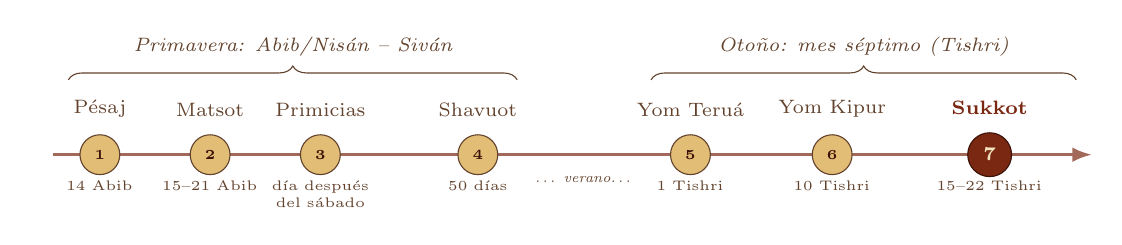
\begin{tikzpicture}[x=1cm,y=1cm,font=\scriptsize]
 \def\fiestaactual{7}
 \draw[line width=1.2pt,tierraroja!70,-{Latex[length=2.5mm]}] (0,0) -- (13.2,0);
 \draw[decorate,decoration={brace,amplitude=5pt},sepia] (0.2,0.95) -- (5.9,0.95) node[midway,above=5pt,font=\scriptsize\itshape]{Primavera: Abib/Nisán -- Siván};
 \draw[decorate,decoration={brace,amplitude=5pt},sepia] (7.6,0.95) -- (13.0,0.95) node[midway,above=5pt,font=\scriptsize\itshape]{Otoño: mes séptimo (Tishri)};
 \foreach \n/\x/\t/\d in {1/0.6/Pésaj/{14 Abib},2/2.0/Matsot/{15--21 Abib},3/3.4/Primicias/{día después del sábado},4/5.4/Shavuot/{50 días},5/8.1/Yom Teruá/{1 Tishri},6/9.9/Yom Kipur/{10 Tishri},7/11.9/Sukkot/{15--22 Tishri}}{
   \ifnum\n=\fiestaactual
     \node[circle,fill=tierraroja,draw=caferojizo,minimum size=5.5mm,text=papiro,font=\scriptsize\bfseries] at (\x,0) {\n};
     \node[above=3pt,font=\scriptsize\bfseries,text=tierraroja] at (\x,0.28) {\t};
   \else
     \node[circle,fill=mostaza!70,draw=sepia,minimum size=4.5mm,text=caferojizo,font=\tiny\bfseries] at (\x,0) {\n};
     \node[above=3pt,text=sepia] at (\x,0.25) {\t};
   \fi
   \node[below=6pt,text width=1.6cm,align=center,font=\tiny,text=sepia] at (\x,0) {\d};}
 \node[font=\tiny\itshape,text=sepia] at (6.75,-0.32) {\ldots\ verano\ldots};
\end{tikzpicture}\par
{\footnotesize\color{sepia}\textit{Figura 1.} El ciclo de Levítico 23. Sukkot (7) dura siete días y lo sigue el Octavo día, \emph{atséret} (22 Tishri). \textit{Nota.} Elaboración propia.}
\end{center}

%===================================================================
\section{El texto: Levítico 23:33--43 y sus paralelos}

\subsection{El texto ancla}
Levítico trata Sukkot en dos bloques. El primero (vv. 33--36) da la fecha, el nombre, los días santos y las ofrendas, con la fórmula que usa para las demás fiestas:

\hebverso{בַּחֲמִשָּׁה עָשָׂר יוֹם לַחֹדֶשׁ הַשְּׁבִיעִי הַזֶּה חַג הַסֻּכּוֹת שִׁבְעַת יָמִים לַיהוָה}
\begin{cita}Y habló \SENOR{} a Moisés, diciendo: Habla a los hijos de Israel y diles: A los quince días de este mes séptimo será la fiesta solemne de los tabernáculos a \SENOR{} por siete días. El primer día habrá santa convocación; ningún trabajo de siervos haréis. Siete días ofreceréis ofrenda encendida a \SENOR; el octavo día tendréis santa convocación, y ofreceréis ofrenda encendida a \SENOR; es fiesta, ningún trabajo de siervos haréis.\fuente{(Lv 23:33--36)}\end{cita}

Donde la RVR1960 dice ``es fiesta'', el hebreo dice \heb{עֲצֶרֶת הִוא} (\emph{atséret hi}), ``es asamblea de clausura'' (véase §4.3). Sigue el colofón de todo el capítulo (``Estas son las fiestas solemnes de \SENOR\ldots'', vv. 37--38) y, ya después de él, una segunda instrucción que solo Sukkot tiene:

\begin{cita}Pero a los quince días del mes séptimo, cuando hayáis recogido el fruto de la tierra, haréis fiesta a \SENOR{} por siete días; el primer día será de reposo, y el octavo día será también día de reposo. Y tomaréis el primer día ramas con fruto de árbol hermoso, ramas de palmeras, ramas de árboles frondosos, y sauces de los arroyos, y os regocijaréis delante de \SENOR{} vuestro Dios por siete días.\fuente{(Lv 23:39--40)}\end{cita}

\hebverso{וּלְקַחְתֶּם לָכֶם בַּיּוֹם הָרִאשׁוֹן פְּרִי עֵץ הָדָר כַּפֹּת תְּמָרִים וַעֲנַף עֵץ־עָבֹת וְעַרְבֵי־נָחַל \\ וּשְׂמַחְתֶּם לִפְנֵי יְהוָה אֱלֹהֵיכֶם שִׁבְעַת יָמִים}

El verso 40 nombra cuatro especies vegetales, ordena tomarlas ``el primer día'' y manda alegrarse ``delante del \SENOR'' durante siete días. Los versos 41--43 cierran con el estatuto perpetuo, la orden de habitar en cabañas y su motivo:

\hebverso{בַּסֻּכֹּת תֵּשְׁבוּ שִׁבְעַת יָמִים כָּל־הָאֶזְרָח בְּיִשְׂרָאֵל יֵשְׁבוּ בַּסֻּכֹּת \\ לְמַעַן יֵדְעוּ דֹרֹתֵיכֶם כִּי בַסֻּכּוֹת הוֹשַׁבְתִּי אֶת־בְּנֵי יִשְׂרָאֵל בְּהוֹצִיאִי אוֹתָם מֵאֶרֶץ מִצְרָיִם}
\begin{cita}Y le haréis fiesta a \SENOR{} por siete días cada año; será estatuto perpetuo por vuestras generaciones; en el mes séptimo la haréis. En tabernáculos habitaréis siete días; todo natural de Israel habitará en tabernáculos, para que sepan vuestros descendientes que en tabernáculos hice yo habitar a los hijos de Israel cuando los saqué de la tierra de Egipto. Yo \SENOR{} vuestro Dios.\fuente{(Lv 23:41--43)}\end{cita}

Tres rasgos distinguen esta fiesta de las otras seis. Es la única con una \destacar{acción doméstica} que dura toda la fiesta, habitar (\heb{יָשַׁב}, \emph{yashav}, ``sentarse, residir'') en la cabaña; la única cuya razón se formula como \destacar{pedagogía de generaciones}, ``para que sepan vuestros descendientes''; y la única con un día añadido después de los siete, con nombre propio. Vale la pena detenerse en el verbo que Dios se atribuye, que es causativo: \heb{הוֹשַׁבְתִּי} (\emph{hoshávti}), ``hice habitar''. Lo que la cabaña recuerda no es lo que Israel construyó, sino dónde Dios lo hizo vivir.

\subsection{Tabla sinóptica}
Seis textos legislativos tratan la fiesta. Cada uno añade algo:

\begin{center}\small\renewcommand{\arraystretch}{1.2}
\begin{tabular}{@{}L{2.4cm}L{3.4cm}L{8.6cm}@{}}
\toprule
\textbf{Texto} & \textbf{Nombre} & \textbf{Qué añade} \\ \midrule
Éx 23:16 & \heb{חַג הָאָסִף} \emph{jag haasif}, ``fiesta de la cosecha'' & Fecha agrícola: ``a la salida del año'' (\heb{בְּצֵאת הַשָּׁנָה}), cuando se recoge el fruto del campo. Una de las tres fiestas de peregrinación (23:14, 17). \\
Éx 34:22 & \emph{jag haasif} & ``A la vuelta del año'' (\heb{תְּקוּפַת הַשָּׁנָה}, trad. propia): el punto en que el año gira. Tres veces al año ``se presentará todo varón'' (34:23). \\
Lv 23:33--43 & \heb{חַג הַסֻּכּוֹת} \emph{jag hasucot} & Fecha exacta (15--21 del mes séptimo), santa convocación el primero y el octavo, \emph{atséret}; cuatro especies; alegría siete días; habitar en cabañas; motivo histórico (el éxodo). \\
Nm 29:12--38 & (sin nombre propio) & Los sacrificios de cada día: 13, 12, 11, 10, 9, 8 y 7 novillos (70 en total), con carneros, corderos y un macho cabrío diario; el octavo día, un solo novillo. \\
Dt 16:13--15 & \heb{חַג הַסֻּכֹּת} \emph{jag hasucot} & Tiempo: ``cuando hayas hecho la cosecha de tu era y de tu lagar''; lugar: ``en el lugar que \SENOR{} escogiere''; inclusión del levita, el extranjero, el huérfano y la viuda; ``estarás verdaderamente alegre''. \\
Dt 31:9--13 & \emph{jag hasucot}, en el año de la \emph{shemitá} & Cada siete años, en Sukkot, lectura pública de la Torá ante todo el pueblo, incluidos niños y extranjeros (\heb{הַקְהֵל}, \emph{haqhel}). \\
\bottomrule
\end{tabular}\par
{\footnotesize\color{sepia}\textit{Tabla 1.} Los textos legislativos de Sukkot. \textit{Nota.} Elaboración propia sobre la RVR1960 y la BHS.}
\end{center}

Leída en orden, la tabla muestra una progresión. El Código de la Alianza (Éx 23; 34) nombra la fiesta por la tarea agrícola; Levítico la vincula con el éxodo y con la cabaña; Números la convierte en calendario de altar; Deuteronomio le da un lugar, una comunidad y un tono, el de la alegría; y Dt 31 le asigna cada siete años una función de catequesis nacional. La serie distingue entre el ``Reglamento del Culto'' (Lv 23), que establece las convocaciones, y ``la Ley de los sacrificios'' (Nm 28--29), que fija los ritos; la tabla respeta esa distinción, pues Lv 23 manda ``ofrenda encendida'' sin detallarla y Nm 29 da el detalle.

\subsection{Propósito y prácticas de la fiesta}
En mi presentación anterior resumí el propósito de Sukkot en tres verbos, cada uno con su texto:

\begin{enumerate}
\item \textbf{Hacer fiesta al \SENOR.} Cada día se ofrecen holocaustos (\heb{עֹלָה}, \emph{olá}), ofrendas de cereal (\heb{מִנְחָה}, \emph{minjá}) con sus libaciones, y un macho cabrío ``por expiación'' (Nm 29:12--38). Antes que nada, la fiesta es culto: ``haréis fiesta a \SENOR'' (Lv 23:39, 41).
\item \textbf{Regocijarse.} La alegría es un mandato motivado por la bendición de la cosecha: ``porque te habrá bendecido \SENOR{} tu Dios en todos tus frutos\ldots{} y estarás verdaderamente alegre'' (Dt 16:13--15).
\item \textbf{Recordar.} Habitar en cabañas ``para que sepan vuestros descendientes'' (Lv 23:43).
\end{enumerate}

A esos propósitos corresponden cinco consideraciones prácticas, tomadas de la misma presentación: habitar siete días en la cabaña, comiendo y durmiendo en ella (Lv 23:42); tomar el primer día las ramas de las cuatro especies (Lv 23:40); guardar el primero y el octavo día como reposo (Lv 23:39); no presentarse con las manos vacías: ``ninguno se presentará delante de \SENOR{} con las manos vacías; cada uno con la ofrenda de su mano, conforme a la bendición que \SENOR{} tu Dios te hubiere dado'' (Dt 16:16--17); y observarla como estatuto perpetuo (Lv 23:41).

\begin{nota}[Precisión]
(1) En los días de Sukkot, Nm 29 llama al macho cabrío \heb{חַטָּאת} (\emph{jatat}), que la RVR1960 traduce ``por expiación''; el verbo \heb{כִּפֶּר} (\emph{kipper}, ``hacer expiación, reconciliar'') aparece en esa serie de ofrendas en las de Trompetas y Expiación (Nm 29:5, 11). La serie ubica estos ritos en ``la Ley de los sacrificios'', distinta del ``Reglamento del Culto'' (§2.2). (2) El texto dice ``habitaréis'' (\heb{תֵּשְׁבוּ}). Que habitar signifique comer y dormir en la cabaña es la interpretación rabínica (``tal como habitáis [en casa], así habitaréis'', b. Sukká 28b), coherente con el sentido del verbo.
\end{nota}

\subsection{Los ocho días y sus sacrificios}
Números 29 asigna a cada día de Sukkot un holocausto propio, además del continuo. El número de novillos baja de uno en uno, mientras los carneros (2), los corderos (14) y el macho cabrío para expiación (1) se mantienen:

\begin{center}
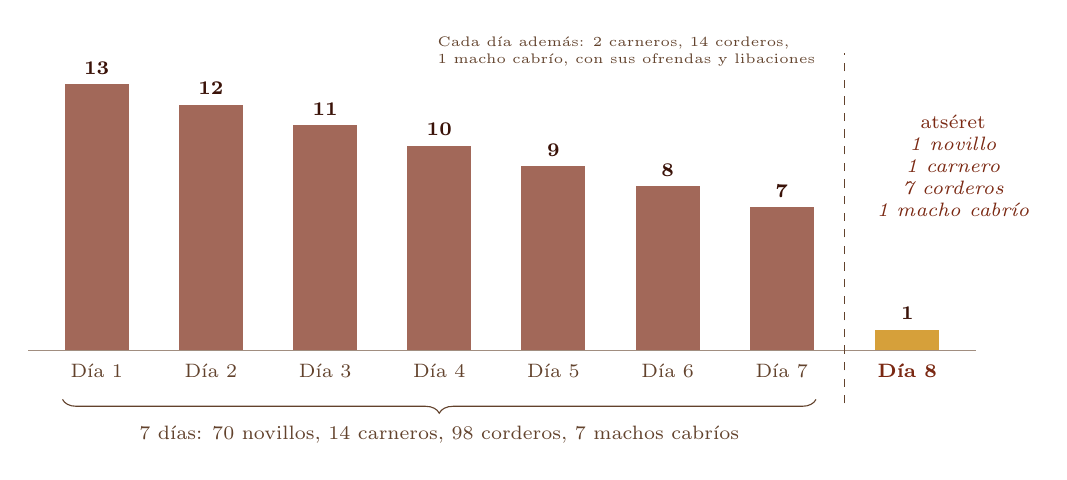
\begin{tikzpicture}[x=1.45cm,y=0.26cm,font=\scriptsize]
 \draw[sepia!60] (0.4,0) -- (8.7,0);
 \foreach \d/\n in {1/13,2/12,3/11,4/10,5/9,6/8,7/7}{
   \fill[tierraroja!70] (\d-0.28,0) rectangle (\d+0.28,\n);
   \node[above,font=\scriptsize\bfseries,text=caferojizo] at (\d,\n) {\n};
   \node[below,text=sepia] at (\d,-0.2) {Día \d};}
 \fill[mostaza] (8.1-0.28,0) rectangle (8.1+0.28,1);
 \node[above,font=\scriptsize\bfseries,text=caferojizo] at (8.1,1) {1};
 \node[below,text=tierraroja,font=\scriptsize\bfseries] at (8.1,-0.2) {Día 8};
 \draw[dashed,sepia] (7.55,-2.6) -- (7.55,14.5);
 \node[text=tierraroja,font=\scriptsize\itshape,align=center] at (8.5,9) {\emph{atséret}\\1 novillo\\1 carnero\\7 corderos\\1 macho cabrío};
 \draw[decorate,decoration={brace,amplitude=5pt,mirror},sepia] (0.7,-2.4) -- (7.3,-2.4) node[midway,below=6pt,text=sepia,align=center]{7 días: 70 novillos, 14 carneros, 98 corderos, 7 machos cabríos};
 \node[text=sepia,font=\tiny,align=left,anchor=west] at (3.9,14.6) {Cada día además: 2 carneros, 14 corderos,\\1 macho cabrío, con sus ofrendas y libaciones};
\end{tikzpicture}\par
{\footnotesize\color{sepia}\textit{Figura 2.} Novillos ofrecidos cada día de Sukkot según Nm 29:12--38. \textit{Nota.} Elaboración propia; sumas propias sobre el texto de Números.}
\end{center}

Todas las cifras son múltiplos de siete: 70 novillos, 14 carneros ($2 \times 7$), 98 corderos ($2 \times 7 \times 7$), 7 machos cabríos, y el séptimo día se ofrecen exactamente siete novillos. El octavo día rompe la serie. Vuelve a las cifras de Yom Teruá y de Yom Kipur (un novillo, un carnero, siete corderos; Nm 29:2, 8, 36) y queda como un día aparte, que Números nombra con la misma palabra que Levítico: ``El octavo día tendréis solemnidad'' (\heb{עֲצֶרֶת תִּהְיֶה לָכֶם}, Nm 29:35).

\begin{nota}[Precisión]
El descenso de 13 a 7 no tiene explicación en el texto. La tradición rabínica relacionó los setenta novillos con las setenta naciones de Génesis 10: ``¿A qué corresponden estos setenta novillos? A las setenta naciones'' (b. Sukká 55b, atribuido a R.\ Eleazar), y el novillo único del octavo día con Israel. Es una interpretación talmúdica, no una afirmación del texto bíblico; se retoma en §6.4 porque coincide con la apertura universal de Zac 14:16 y de 1~R 8:41--43. Otras explicaciones son de orden práctico, como la disminución progresiva al final de una fiesta larga (Milgrom, 1990; Levine, 1989).
\end{nota}

\subsection{Cada siete años: la lectura de la Torá}
Deuteronomio asigna a Sukkot una tarea que ninguna otra fiesta tiene, la lectura pública de la Ley en el año de la remisión.

\hebverso{מִקֵּץ שֶׁבַע שָׁנִים בְּמֹעֵד שְׁנַת הַשְּׁמִטָּה בְּחַג הַסֻּכּוֹת}
\begin{cita}Al fin de cada siete años, en el año de la remisión, en la fiesta de los tabernáculos, cuando viniere todo Israel a presentarse delante de \SENOR{} tu Dios en el lugar que él escogiere, leerás esta ley delante de todo Israel a oídos de ellos. Harás congregar al pueblo, varones y mujeres y niños, y tus extranjeros que estuvieren en tus ciudades, para que oigan y aprendan, y teman a \SENOR{} vuestro Dios, y cuiden de cumplir todas las palabras de esta ley.\fuente{(Dt 31:10--12)}\end{cita}

La palabra \heb{הַקְהֵל} (\emph{haqhel}, ``congrega'') dio nombre a la ceremonia. Importa dónde cae en el calendario: la lectura se hace en la fiesta de la abundancia, en el año en que la tierra descansó y las deudas se remitieron, de modo que el pueblo oye la Ley después de haber experimentado durante un año entero que vive de lo que Dios da y no solo de lo que produce. El estudio 08 de la serie desarrolla el ciclo de la \emph{shemitá}; aquí basta ubicar Sukkot dentro de él:

\begin{center}
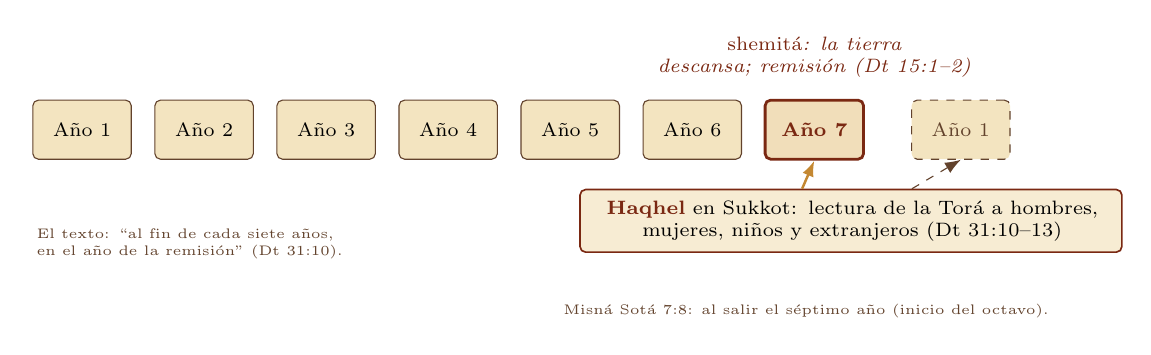
\begin{tikzpicture}[x=1.55cm,y=1cm,font=\scriptsize]
 \foreach \a in {1,...,6}{
   \node[draw=sepia,fill=papiro,minimum width=1.25cm,minimum height=0.75cm,rounded corners=2pt] at (\a,0) {Año \a};}
 \node[draw=tierraroja,line width=1pt,fill=mostaza!35,minimum width=1.25cm,minimum height=0.75cm,rounded corners=2pt,font=\scriptsize\bfseries,text=tierraroja] (a7) at (7,0) {Año 7};
 \node[draw=sepia,dashed,fill=papiro,minimum width=1.25cm,minimum height=0.75cm,rounded corners=2pt,text=sepia] (a8) at (8.2,0) {Año 1};
 \node[above=4pt,text=tierraroja,font=\scriptsize\itshape,align=center] at (7,0.4) {\emph{shemitá}: la tierra\\descansa; remisión (Dt 15:1--2)};
 \node[caja,below=0.75cm,text width=6.6cm,align=center] (h) at (7.3,0) {\textbf{\textcolor{tierraroja}{Haqhel}} en Sukkot: lectura de la Torá a hombres, mujeres, niños y extranjeros (Dt 31:10--13)};
 \draw[-{Latex[length=2mm]},mostaza!80!tierraroja,line width=0.9pt] (h.north) ++(-0.4,0) -- (a7.south);
 \draw[-{Latex[length=2mm]},sepia,dashed] (h.north) ++(0.5,0) -- (a8.south);
 \node[text=sepia,font=\tiny,align=left,anchor=west] at (0.55,-1.45) {El texto: ``al fin de cada siete años,\\en el año de la remisión'' (Dt 31:10).};
 \node[text=sepia,font=\tiny,align=right,anchor=east] at (9.0,-2.3) {Misná Sotá 7:8: al salir el séptimo año (inicio del octavo).};
\end{tikzpicture}\par
{\footnotesize\color{sepia}\textit{Figura 3.} \emph{Haqhel} dentro del ciclo de siete años. \textit{Nota.} Elaboración propia; la ubicación al inicio del octavo año es la interpretación de la Misná.}
\end{center}

\begin{nota}[Precisión]
El texto dice ``al fin de cada siete años, en el año de la remisión''. La Misná entiende que la lectura se hacía en el Sukkot que abre el año siguiente a la \emph{shemitá} y describe al rey leyendo desde una tarima en el atrio; narra que Agripa leyó de pie y lloró al llegar a ``no podrás poner sobre ti a hombre extranjero'' (Dt 17:15), y que el pueblo le respondió: ``Tú eres nuestro hermano'' (Misná Sotá 7:8). Es un testimonio de la práctica del Segundo Templo según la tradición rabínica, no del período bíblico. Neh 8 muestra una lectura pública en el mes séptimo, pero no dice que fuera año de \emph{shemitá}.
\end{nota}

%===================================================================
\section{Lectura histórica}

\subsection{La cosecha final y el giro del año}
En el clima de Israel el año agrícola tiene dos tiempos. La cebada madura en primavera (Pésaj y Primicias) y el trigo a comienzos del verano (Shavuot); después vienen los meses secos, en que maduran la uva, el higo, la granada y la aceituna. El mes séptimo (septiembre--octubre) cierra ese ciclo, con la uva pisada, el aceite prensado y el grano trillado. Por eso Deuteronomio fecha la fiesta ``cuando hayas hecho la cosecha de tu era y de tu lagar'' (Dt 16:13) y Éxodo la llama \emph{jag haasif}, ``fiesta de la recolección'' (Éx 23:16). Lo que sigue en el año depende de las primeras lluvias, la \emph{yoré} (Dt 11:14; Jl 2:23), que ablandan la tierra para arar y sembrar. La fiesta queda entre lo recogido y lo que se espera.

Esa posición explica dos rasgos posteriores. La Misná dice que ``en la Fiesta [el mundo] es juzgado respecto del agua'' (Misná Rosh haShaná 1:2) y discute desde cuándo se menciona la lluvia en la oración diaria: R.\ Eliezer, desde el primer día festivo de la Fiesta; R.\ Josué, cuya opinión prevaleció, desde el último (Misná Taanit 1:1). Zacarías amenaza con la falta de lluvia a las naciones que no suban a celebrar Sukkot (Zac 14:17), y la libación del agua del Segundo Templo (§3.4) pertenece al mismo horizonte.

La fecha, el 15 del mes, coincide con la luna llena, como en Matsot (15 de Abib). Las dos fiestas de siete días están en espejo, a seis meses de distancia: una abre el año de las cosechas y la otra lo cierra. Éx 34:22 dice que la fiesta cae ``a la vuelta del año'' (\emph{tequfat hashaná}), y Éx 23:16 ``a la salida del año'' (\emph{betset hashaná}). Las dos expresiones describen el giro del año agrícola en otoño, cerca del equinoccio, y no implican que el año del calendario cultual empiece en Tishri (Éx 12:2 lo hace empezar en Abib).

\begin{nota}[Precisión]
Muchos autores ven en las chozas que los agricultores levantaban en viñas y huertos durante la vendimia (cf. Is 1:8, ``como enramada en viña''; Job 27:18) el origen práctico de la cabaña festiva, y en la fiesta de Silo ``en las viñas'' (Jue 21:19--21; cf. 1~S 1:3) una celebración de vendimia del período de los jueces (de Vaux, 1985). Es una hipótesis histórica razonable, pero el texto bíblico da otra razón, histórica y teológica: el éxodo (Lv 23:43). Los paralelos de fiestas de cosecha en el antiguo Cercano Oriente son generales y no explican el rasgo propio de Israel: la memoria del desierto.
\end{nota}

\subsection{La \emph{sucá}: una casa que no dura}
La Torá no describe cómo se construye la cabaña. Neh 8:15--16 muestra que se hacía con ramas y se levantaba en las azoteas, en los patios, en los atrios del templo y en las plazas; la Misná dedica los dos primeros capítulos del tratado Sukká a definirla. Sus normas principales son estas:

\begin{center}
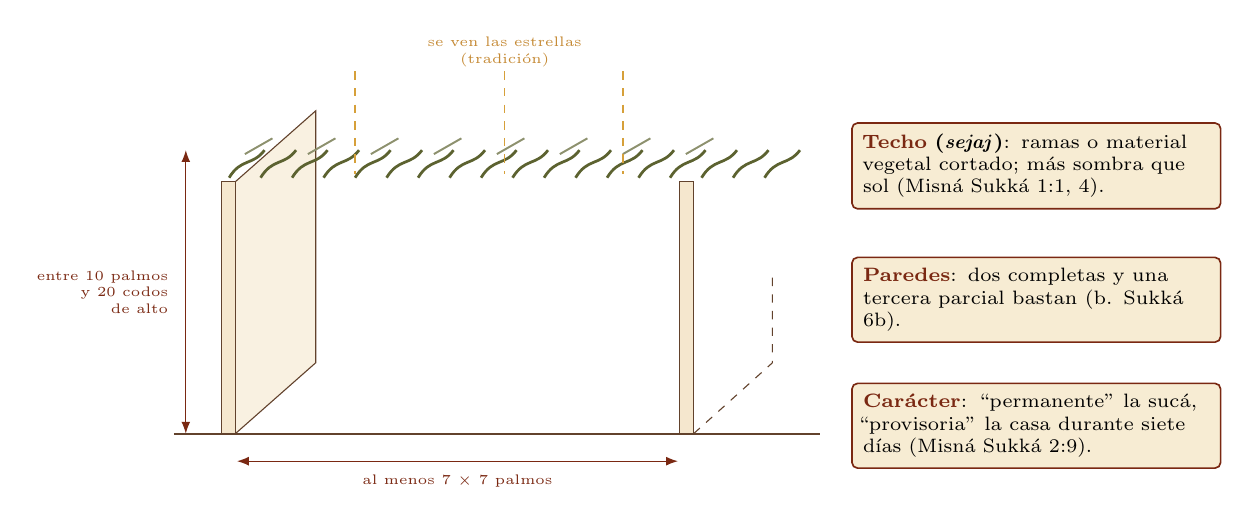
\begin{tikzpicture}[x=1cm,y=1cm,font=\scriptsize]
 % suelo
 \draw[sepia,line width=0.8pt] (-0.6,0) -- (7.6,0);
 % paredes
 \fill[mostaza!25] (0,0) rectangle (0.18,3.2);
 \fill[mostaza!25] (5.82,0) rectangle (6,3.2);
 \fill[mostaza!15] (0.18,0) -- (1.2,0.9) -- (1.2,4.1) -- (0.18,3.2) -- cycle;
 \draw[sepia] (0,0) rectangle (0.18,3.2) (5.82,0) rectangle (6,3.2);
 \draw[sepia] (0.18,0) -- (1.2,0.9) -- (1.2,4.1) -- (0.18,3.2);
 \draw[sepia,dashed] (6,0) -- (7.0,0.9) -- (7.0,2.0);
 % techo de ramas
 \foreach \x in {0.1,0.5,...,6.9}{
   \draw[oliva,line width=1pt] (\x,3.25) .. controls (\x+0.15,3.5) and (\x+0.3,3.4) .. (\x+0.45,3.6);}
 \foreach \x in {0.3,1.1,...,6.5}{
   \draw[oliva!70,line width=0.7pt] (\x,3.55) -- (\x+0.35,3.75);}
 % rayos de luz entre ramas
 \foreach \x in {1.7,3.6,5.1}{\draw[mostaza,line width=0.5pt,dashed] (\x,4.6) -- (\x,3.3);}
 \node[mostaza!80!tierraroja,font=\tiny,align=center] at (3.6,4.85) {se ven las estrellas\\(tradición)};
 % cotas
 \draw[{Latex[length=1.5mm]}-{Latex[length=1.5mm]},tierraroja] (-0.45,0) -- (-0.45,3.6);
 \node[text=tierraroja,font=\tiny,align=right,anchor=east] at (-0.55,1.8) {entre 10 palmos\\y 20 codos\\de alto};
 \draw[{Latex[length=1.5mm]}-{Latex[length=1.5mm]},tierraroja] (0.2,-0.35) -- (5.8,-0.35);
 \node[text=tierraroja,font=\tiny,below] at (3,-0.4) {al menos 7 $\times$ 7 palmos};
 % rótulos
 \node[caja,anchor=west,text width=4.4cm] at (8.0,3.4) {\textbf{\textcolor{tierraroja}{Techo} (\emph{sejaj})}: ramas o material vegetal cortado; más sombra que sol (Misná Sukká 1:1, 4).};
 \node[caja,anchor=west,text width=4.4cm] at (8.0,1.7) {\textbf{\textcolor{tierraroja}{Paredes}}: dos completas y una tercera parcial bastan (b. Sukká 6b).};
 \node[caja,anchor=west,text width=4.4cm] at (8.0,0.1) {\textbf{\textcolor{tierraroja}{Carácter}}: ``permanente'' la sucá, ``provisoria'' la casa durante siete días (Misná Sukká 2:9).};
\end{tikzpicture}\par
{\footnotesize\color{sepia}\textit{Figura 4.} Esquema de una \emph{sucá} según la Misná. \textit{Nota.} Elaboración propia. Medidas y normas rabínicas (Misná y Talmud), no bíblicas.}
\end{center}

La norma que mejor resume el sentido de la cabaña está en Misná Sukká 2:9: ``Durante los siete días, la persona hace de su sucá su morada fija y de su casa su morada provisoria''. Durante una semana se invierte la relación normal entre lo durable y lo pasajero. La misma Misná añade una imagen para la lluvia que obliga a dejar la cabaña, la de un siervo que viene a servir la copa a su amo y recibe el agua en la cara; la lluvia en Sukkot se leía como señal de desagrado.

\begin{nota}[Precisión]
Las medidas (altura mínima de diez palmos y máxima de veinte codos, al menos siete por siete palmos), la proporción de sombra y sol, el número de paredes y el material del techo son \emph{halajá} rabínica (Misná Sukká 1--2; b. Sukká 2a--7b). La Torá solo manda ``habitar en cabañas''. Que el techo deje ver las estrellas es costumbre posterior, deducida de esas normas.
\end{nota}

\subsection{La fiesta en la historia narrada de Israel}
La historia bíblica menciona Sukkot en momentos de fundación y de refundación.

\textbf{La dedicación del templo.} Salomón dedicó el templo ``en el mes de Etanim, que es el mes séptimo, en el día de la fiesta solemne'' (1~R 8:2). La nube llenó la casa (8:10--11), y Salomón oró también por el extranjero que viniera ``de lejanas tierras a causa de tu nombre'' (8:41--43). El relato termina con alegría de fiesta:

\begin{cita}Y al octavo día despidió al pueblo; y ellos, bendiciendo al rey, se fueron a sus moradas alegres y gozosos de corazón, por todos los beneficios que \SENOR{} había hecho a David su siervo y a su pueblo Israel.\fuente{(1~R 8:66)}\end{cita}

Reyes habla de ``siete días y aun por otros siete días, esto es, por catorce días'' (8:65). Crónicas ordena los datos según Levítico: siete días de dedicación del altar, siete días de fiesta, ``al octavo día hicieron solemne asamblea'' (\emph{atséret}) y el pueblo vuelve a casa el día 23 (2~Cr 7:7--10). Crónicas anota además que todos los sacerdotes presentes se habían santificado sin atenerse a sus turnos (2~Cr 5:11): la dedicación reunió a todo el sacerdocio, y la consagración del templo quedó terminada en Sukkot. En la fiesta de las cabañas, la morada de Dios en tienda pasa a ser morada en casa de piedra.

\textbf{La fiesta de Jeroboam.} Al dividirse el reino, Jeroboam instituyó en Betel una fiesta ``en el mes octavo, a los quince días del mes, conforme a la fiesta solemne que se celebraba en Judá''; el narrador la califica como ``el mes que él había inventado de su propio corazón'' (1~R 12:32--33). Es la primera alteración deliberada del calendario bíblico, y el relato la presenta como parte del pecado que marcó al reino del norte. Ilustra una tesis que recorre toda la serie: las fiestas son ``de \SENOR'' y no se trasladan por conveniencia política.

\textbf{El regreso del destierro.} Lo primero que celebran los repatriados, antes de poner los cimientos del templo, es Sukkot: ``Celebraron asimismo la fiesta solemne de los tabernáculos, como está escrito, y holocaustos cada día por orden conforme al rito, cada cosa en su día'' (Esd 3:4). La serie usa este verso para distinguir el ``Reglamento del Culto'' (``como está escrito'') de ``la Ley de los sacrificios'' (``conforme al rito''). Una generación después, la lectura de la Ley por Esdras en el mes séptimo lleva al pueblo a redescubrir el mandato de las cabañas:

\begin{cita}Y toda la congregación que volvió de la cautividad hizo tabernáculos, y en tabernáculos habitó; porque desde los días de Josué hijo de Nun hasta aquel día, no habían hecho así los hijos de Israel. Y hubo alegría muy grande. Y leyó Esdras en el libro de la ley de Dios cada día, desde el primer día hasta el último; e hicieron la fiesta solemne por siete días, y el octavo día fue de solemne asamblea, según el rito.\fuente{(Neh 8:17--18)}\end{cita}

``Desde los días de Josué hijo de Nun'' no puede significar que la fiesta no se celebrara nunca (cf. 1~R 8; Esd 3:4). Los comentaristas entienden que no se había hecho ``así'', con toda la comunidad viviendo en cabañas, con esa alegría y con lectura diaria de la Ley (Rubenstein, 1995). El dato interesa a la serie porque es el único texto que une de manera explícita Sukkot con la generación de Josué, la que entró en la tierra.

\textbf{La fiesta en los profetas.} Oseas anuncia un regreso al desierto que es castigo y nuevo comienzo a la vez: ``aún te haré morar en tiendas, como en los días de la fiesta'' (Os 12:9 [12:10]). Zacarías ve, al final, a las naciones que suben ``de año en año'' a Jerusalén para adorar al Rey y celebrar la fiesta de los tabernáculos (Zac 14:16). Ezequiel 45:25 fija las ofrendas del príncipe en el templo futuro: ``En el mes séptimo, a los quince días del mes, en la fiesta, hará como en estos siete días''.

\begin{center}
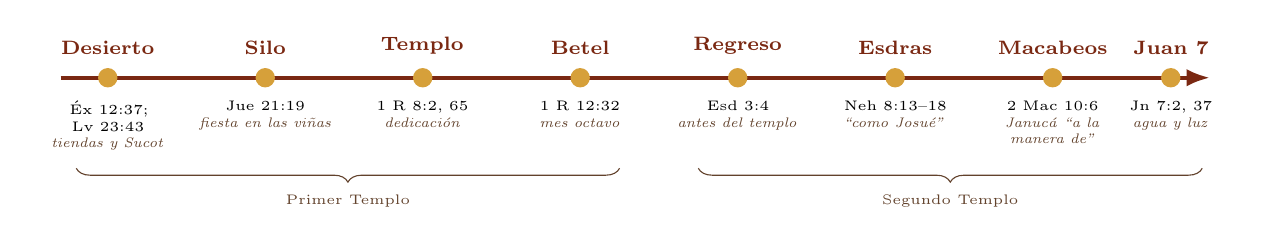
\begin{tikzpicture}[font=\scriptsize]
 \draw[line width=1.6pt,tierraroja,-{Latex[length=3mm]}] (0,0) -- (14.6,0);
 \foreach \x/\a/\b/\c in {0.6/{Desierto}/{Éx 12:37; Lv 23:43}/{tiendas y Sucot}, 2.6/{Silo}/{Jue 21:19}/{fiesta en las viñas}, 4.6/{Templo}/{1 R 8:2, 65}/{dedicación}, 6.6/{Betel}/{1 R 12:32}/{mes octavo}, 8.6/{Regreso}/{Esd 3:4}/{antes del templo}, 10.6/{Esdras}/{Neh 8:13--18}/{``como Josué''}, 12.6/{Macabeos}/{2 Mac 10:6}/{Janucá ``a la manera de''}, 14.1/{Juan 7}/{Jn 7:2, 37}/{agua y luz}}{
   \fill[mostaza] (\x,0) circle (3.5pt);
   \node[above=5pt,font=\scriptsize\bfseries,text=tierraroja,text width=1.8cm,align=center] at (\x,0) {\a};
   \node[below=5pt,text width=1.8cm,align=center,font=\tiny] at (\x,0) {\b\\\textit{\color{sepia}\c}};}
 \draw[decorate,decoration={brace,amplitude=5pt,mirror},sepia] (0.2,-1.15) -- (7.1,-1.15) node[midway,below=6pt,font=\tiny,text=sepia]{Primer Templo};
 \draw[decorate,decoration={brace,amplitude=5pt,mirror},sepia] (8.1,-1.15) -- (14.5,-1.15) node[midway,below=6pt,font=\tiny,text=sepia]{Segundo Templo};
\end{tikzpicture}\par
{\footnotesize\color{sepia}\textit{Figura 5.} Sukkot en la historia narrada de Israel. \textit{Nota.} Elaboración propia. La identificación de la fiesta de Silo con Sukkot es probable, no explícita.}
\end{center}

\subsection{Sukkot en el Segundo Templo}
En los siglos anteriores a Jesús, Sukkot era la fiesta de peregrinación más concurrida. Josefo la llama ``la fiesta más santa y más grande entre los hebreos'' (\emph{Ant.} 8.100, a propósito de la dedicación salomónica) y describe sus ritos: habitar en tiendas, llevar en la mano un ramo de mirto y sauce con una rama de palmera y el fruto de la \emph{persea}, y los sacrificios de cada día (\emph{Ant.} 3.244--247). Filón la explica como fiesta de la cosecha completa y memoria de la vida en el desierto, que enseña la igualdad entre ricos y pobres (\emph{De specialibus legibus} 2; Filón, 1937).

Otras fuentes muestran el peso nacional que había adquirido:

\begin{itemize}
\item El libro de los \textbf{Jubileos} (s.~II a.\,e.\,c.) atribuye a Abraham la primera celebración de Sukkot en Beerseba, con cabañas y ramas, y la presenta como ordenanza eterna (Jub 16:20--31; Charlesworth, 1985). Es una relectura del Segundo Templo, pero coincide con el interés de la serie por Abraham, que vivió ``en tiendas'' (He 11:9).
\item \textbf{2 Macabeos} narra que, al purificar el templo en el mes de Kislev (164 a.\,e.\,c.), los judíos ``celebraron con alegría ocho días, a la manera de la fiesta de las cabañas'', recordando que poco antes habían pasado esa fiesta escondidos en montes y cuevas ``como fieras''; llevaban ramas y palmas (2~Mac 10:6--7; cf. 1:9). Janucá nació así como un Sukkot diferido; Juan menciona esa fiesta: ``Celebrábase en Jerusalén la fiesta de la dedicación'' (Jn 10:22).
\item \textbf{1 Macabeos} describe la entrada de Simón en la ciudadela de Jerusalén ``con alabanzas y ramos de palmera'' (1~Mac 13:51); las palmas eran ya signo de victoria y de entrada triunfal.
\item El \textbf{Rollo del Templo} de Qumrán prescribe cabañas sobre la azotea del atrio del templo ideal para los ancianos y jefes del pueblo durante la fiesta (11QT 42:10--17; Yadin, 1983).
\item \textbf{Josefo} narra que Alejandro Janeo, rey y sumo sacerdote, fue atacado por la multitud con cidras (\emph{etroguim}) mientras oficiaba en el altar durante la fiesta (\emph{Ant.} 13.372), y que el joven sumo sacerdote Aristóbulo III, aclamado por el pueblo en Sukkot, fue ahogado poco después por orden de Herodes (\emph{Ant.} 15.50--56).
\end{itemize}

La Misná, redactada hacia el 200 e.\,c., conserva la memoria de tres ritos del templo que no están en la Torá y que forman el trasfondo inmediato de Juan 7--8.

\textbf{La libación del agua.} Cada mañana de los siete días, un sacerdote llenaba en el estanque de Siloé un jarro de oro con agua; la procesión entraba por la Puerta de las Aguas con toque de \emph{shofar}, y el agua se derramaba en una de dos copas de plata sobre el altar, junto con el vino de la libación (Misná Sukká 4:9). La misma Misná recuerda que una vez un sacerdote derramó el agua sobre sus pies y el pueblo lo apedreó con sus cidras; el Talmud lo identifica con un saduceo (b. Sukká 48b), y Josefo cuenta el episodio de Janeo. El rito era discutido y, quizá por lo mismo, popular.

\textbf{La alegría de la casa de la extracción} (\emph{Simjat Beit haShoevá}). Las noches de la fiesta, en el atrio de las mujeres, se encendían cuatro grandes candelabros de oro, con mechas hechas de las vestiduras gastadas de los sacerdotes, ``y no había patio en Jerusalén que no se iluminara con la luz de la casa de la extracción''; hombres piadosos danzaban con antorchas, y los levitas tocaban sobre los quince escalones que bajaban al atrio, que la tradición relaciona con los quince Cánticos graduales (Sal 120--134). La Misná lo resume en una frase:

\begin{cita}Quien no ha visto la alegría de la casa de la extracción del agua no ha visto alegría en su vida.\fuente{(Misná Sukká 5:1, trad. propia)}\end{cita}

Al amanecer, los sacerdotes bajaban hasta la puerta oriental, se volvían hacia el santuario y decían: ``Nuestros padres, que estuvieron en este lugar, tenían sus espaldas hacia el templo y sus rostros hacia el oriente, y se postraban hacia el oriente ante el sol (Ez 8:16); pero nosotros, nuestros ojos son para Yah'' (Misná Sukká 5:2--4).

\textbf{Los sauces y el ``Hosanna''.} Cada día se colocaban grandes ramas de sauce traídas de Motsá junto al altar, y los sacerdotes daban una vuelta alrededor de él diciendo ``Ana \SENOR, \emph{hoshía na}'' (``sálvanos ahora'', Sal 118:25); el séptimo día daban siete vueltas (Misná Sukká 4:5). En la sinagoga, la gente agitaba el ramo (lulav) al recitar el Hallel, en ``Alabad'' y en ``sálvanos ahora'' (Misná Sukká 3:9). De ahí el nombre posterior del séptimo día, \emph{Hoshaná Rabá}, ``el gran Hosanna''.

\begin{nota}[Precisión]
La Misná es posterior a la destrucción del templo (70 e.\,c.) y describe el culto según la memoria rabínica; parte puede idealizar. Aun así, la libación del agua está confirmada por Josefo y la disputa con los saduceos encaja en lo que se sabe del período. Que el nombre ``casa de la extracción'' derive de Is 12:3 (``Sacaréis con gozo aguas de las fuentes de la salvación'') y que de allí se ``extrajera el Espíritu Santo'' es una interpretación del Talmud de Jerusalén (y. Sukká 5:1, 55a). El término \emph{Hoshaná Rabá} no aparece en la Misná, que describe el séptimo día como el día de las siete vueltas con el sauce (4:5--6). Sobre el uso de estas fuentes para leer Juan, véase Keener (2003) y Rubenstein (1995).
\end{nota}

%===================================================================
\section{Lectura filológica}

\subsection{La cabaña y la tienda}
El nombre de la fiesta es un plural, \heb{סֻכּוֹת} (\emph{sucot}), ``cabañas''. El hebreo tiene tres palabras principales para la morada, y las tres convergen en griego en una sola.

\begin{filologia}[\heb{סֻכָּה} \emph{sucá}, pl.\ \heb{סֻכּוֹת} \emph{sucot}]
\textbf{Raíz} \heb{סכך} (\emph{s-k-k}): ``cubrir, resguardar, entretejer''. Los querubines ``cubren'' el propiciatorio con sus alas (\heb{סֹכְכִים}, Éx 25:20); Dios ``te cubrirá'' con sus plumas (\heb{יָסֶךְ לָךְ}, Sal 91:4); el salmista dice ``me hiciste en el vientre de mi madre'' con un verbo de tejido (\heb{תְּסֻכֵּנִי}, Sal 139:13). La \emph{sucá} es, por su raíz, un techo entretejido que da sombra.\par\smallskip
\textbf{Strong H5521}: femenino de H5520 \heb{סֹךְ} (\emph{sok}), ``espesura, guarida'' (la guarida del león, Jer 25:38). En el Códice de Leningrado \emph{sucá} aparece 31 veces y \emph{sok} 4 (Sal 10:9; 27:5; 76:2 [76:3]; Jer 25:38) (conteo con números Strong). En mi presentación anterior reuní sus traducciones: choza, guarida, cabaña, enramada, escondedero, morada, abrigo, tabernáculo, tienda. El sentido principal es el de una \destacar{morada frágil y temporal}, como la existencia humana (2~Co 5:1).\par\smallskip
\textbf{Usos concretos.} Cabañas para el ganado (Gn 33:17, origen del topónimo Sucot); la primera etapa del éxodo, ``de Ramesés a Sucot'' (Éx 12:37); la enramada del guarda en la viña (Is 1:8); la enramada de Jonás (Jon 4:5); las tiendas del campamento militar: ``El arca e Israel y Judá están bajo tiendas'' (\heb{בַּסֻּכּוֹת}, 2~S 11:11); el abrigo ``para sombra contra el calor del día'' (Is 4:6).\par\smallskip
\textbf{Usos teológicos.} con la forma masculina \heb{סֹךְ} (\emph{sok}): ``Porque él me esconderá en su tabernáculo en el día del mal'' (\heb{בְּסֻכֹּה}, Sal 27:5); ``En Salem está su tabernáculo'' (\heb{סֻכּוֹ}, Sal 76:2 [76:3]); y con \emph{sucá}: ``En aquel día yo levantaré el tabernáculo caído de David'' (\heb{סֻכַּת דָּוִיד הַנֹּפֶלֶת}, Am 9:11), citado por Santiago en Hch 15:16 como \grc{τὴν σκηνὴν Δαυὶδ τὴν πεπτωκυῖαν}. La casa de David, caída, se describe como una choza que Dios volverá a levantar.\par\smallskip
\textbf{LXX:} \grc{σκηνή} (``tienda''); la fiesta es \grc{ἑορτὴ σκηνῶν} (Lv 23:34) o \grc{σκηνοπηγία} (Dt 16:16).
\end{filologia}

\begin{filologia}[\heb{אֹהֶל} \emph{ohel} y \heb{מִשְׁכָּן} \emph{mishkán}]
\heb{אֹהֶל} (\emph{ohel}) es la tienda de pieles o tela del nómada: la de Abraham en el encinar de Mamre (Gn 18:1), la ``tienda de reunión'' (\heb{אֹהֶל מוֹעֵד}, \emph{ohel moed}, Éx 33:7). Oseas promete: ``aún te haré morar en tiendas'' (\heb{בָאֳהָלִים}, Os 12:9 [12:10]).\par\smallskip
\heb{מִשְׁכָּן} (\emph{mishkán}) viene de \heb{שָׁכַן} (\emph{shakhan}), ``habitar, morar, establecerse''. Es el santuario como lugar donde Dios mora: ``Y harán un santuario para mí, y habitaré (\heb{וְשָׁכַנְתִּי}) en medio de ellos'' (Éx 25:8); ``pondré mi morada (\heb{מִשְׁכָּנִי}) en medio de vosotros'' (Lv 26:11); ``Estará en medio de ellos mi tabernáculo'' (Ez 37:27).\par\smallskip
La palabra \heb{שְׁכִינָה} (\emph{shejiná}), ``la presencia que mora'', no aparece en la Biblia hebrea: es término de los targumim y de la literatura rabínica para la presencia de Dios. Su uso para leer Jn 1:14 (``vimos su gloria'') es una analogía legítima, pero posterior.\par\smallskip
\textbf{LXX:} \grc{σκηνή} traduce tanto \emph{ohel} como \emph{mishkán}, y también \emph{sucá}. Algunos intérpretes ven una asonancia entre \grc{σκηνή}/\grc{σκηνόω} y la raíz hebrea \emph{sh-k-n}; es una coincidencia fonética que el griego bíblico pudo aprovechar, no una etimología.
\end{filologia}

\begin{filologia}[\heb{עֲצֶרֶת} \emph{atséret}]
\textbf{Raíz} \heb{עצר} (\emph{'-ts-r}): ``detener, retener, cerrar''. Saray dice ``\SENOR{} me ha hecho estéril'', literalmente ``me ha cerrado'' (\heb{עֲצָרַנִי}, Gn 16:2); Elías avisa a Acab que baje ``para que la lluvia no te ataje'' (1~R 18:44).\par\smallskip
\textbf{Uso cultual.} \emph{Atséret} es la asamblea en que el pueblo se detiene de sus trabajos y queda reunido: el octavo día de Sukkot (Lv 23:36; Nm 29:35; Neh 8:18; 2~Cr 7:9) y el séptimo día de Matsot (Dt 16:8). También se usa para asambleas convocadas en crisis (``convocad a asamblea'', Jl 1:14) o reprobadas (Is 1:13; Am 5:21; la asamblea de Jehú para Baal, 2~R 10:20). La RVR1960 traduce ``es fiesta'' (Lv 23:36), ``solemnidad'' (Nm 29:35) o ``solemne asamblea'' (Neh 8:18).\par\smallskip
\textbf{LXX:} \grc{ἐξόδιον} (Lv 23:36; Nm 29:35; Dt 16:8): ``fiesta de salida, de clausura''.\par\smallskip
\textbf{Tradición:} Rashi, siguiendo el midrash, lee la raíz como ``retener'': Dios dice a Israel, como un rey que invitó a sus hijos a un banquete, ``os he retenido conmigo'': ``vuestra partida me es difícil; quedaos un día más'' (Rashi a Lv 23:36; cf. b. Sukká 55b). Es una lectura homilética de la raíz.
\end{filologia}

\begin{filologia}[\heb{אָסִף} \emph{asif}; \heb{תְּקוּפָה} \emph{tequfá}]
\heb{חַג הָאָסִף} (\emph{jag haasif}), ``fiesta de la recolección'' (Éx 23:16; 34:22). La raíz \heb{אסף} (\emph{'-s-f}) es ``juntar, recoger'': se recoge el fruto, se congrega a las personas y se dice del que muere que ``fue unido a su pueblo'' (\heb{וַיֵּאָסֶף אֶל־עַמָּיו}, Gn 25:8). La fiesta del fin de la cosecha lleva el verbo de los finales.\par\smallskip
\heb{תְּקוּפַת הַשָּׁנָה} (\emph{tequfat hashaná}, Éx 34:22), de \heb{נקף} ``girar, rodear'': ``la vuelta del año'' (cf. \heb{לִתְקֻפוֹת הַיָּמִים}, ``al cumplirse el tiempo'', 1~S 1:20; el ``curso'' del sol, Sal 19:6 [19:7]). \heb{בְּצֵאת הַשָּׁנָה} (\emph{betset hashaná}, Éx 23:16): ``a la salida del año'', el momento en que el año agrícola se cierra.
\end{filologia}

\subsection{Las cuatro especies}
Lv 23:40 nombra cuatro elementos vegetales. Los nombres rabínicos que hoy los identifican (\emph{etrog}, \emph{lulav}, \emph{hadás}, \emph{aravá}) son posteriores; el texto bíblico describe más que nombra:

\begin{center}\small\renewcommand{\arraystretch}{1.25}
\begin{tabular}{@{}L{3.2cm}L{3.6cm}L{3.4cm}L{4.2cm}@{}}
\toprule
\textbf{Hebreo (Lv 23:40)} & \textbf{Literal} & \textbf{RVR1960} & \textbf{Identificación posterior} \\ \midrule
\heb{פְּרִי עֵץ הָדָר} \emph{perí ets hadar} & ``fruto de árbol de esplendor'' & ``ramas con fruto de árbol hermoso'' & \emph{etrog}, cidra (Targum Onkelos; Josefo, \emph{Ant.} 13.372) \\
\heb{כַּפֹּת תְּמָרִים} \emph{kapot temarim} & ``palmas (hojas) de palmeras'' & ``ramas de palmeras'' & \emph{lulav}, el brote cerrado de la palmera datilera \\
\heb{עֲנַף עֵץ־עָבֹת} \emph{anaf ets avot} & ``rama de árbol frondoso, de follaje espeso'' & ``ramas de árboles frondosos'' & \emph{hadás}, mirto (b. Sukká 32b) \\
\heb{עַרְבֵי־נָחַל} \emph{arvé najal} & ``sauces del torrente'' & ``sauces de los arroyos'' & \emph{aravá}, sauce de río (cf. Sal 137:2; Is 44:4) \\
\bottomrule
\end{tabular}\par
{\footnotesize\color{sepia}\textit{Tabla 2.} Las cuatro especies de Lv 23:40. \textit{Nota.} Elaboración propia. La identificación de la columna derecha es rabínica y del Segundo Templo.}
\end{center}

\begin{filologia}[\heb{הָדָר} \emph{hadar}; \emph{lulav}; \emph{etrog}]
\heb{הָדָר} (\emph{hadar}) es ``esplendor, majestad'': ``Alabanza y magnificencia (\heb{הוֹד־וְהָדָר}) delante de él'' (Sal 96:6). ``Fruto de árbol de esplendor'' no nombra una especie, sino una calidad. El Talmud discute el sentido y propone, con un juego de palabras, el árbol cuyo fruto ``habita'' (\emph{ha-dar}) en él todo el año (b. Sukká 35a); Josefo ya supone la cidra.\par\smallskip
\heb{לוּלָב} (\emph{lulav}) y \heb{אֶתְרוֹג} (\emph{etrog}) son términos de la Misná. \emph{Lulav} es el ``brote'' de la palmera; \emph{etrog} parece un préstamo del persa. Atar juntos el lulav, tres ramas de mirto y dos de sauce, y tomarlos con el etrog, es práctica rabínica (Misná Sukká 3), y en ella Lv 23:40 se lee como ``tomad en la mano''. Las monedas de la revuelta de Bar Kojba (132--135 e.\,c.) muestran el lulav y el etrog como emblemas nacionales.
\end{filologia}

\begin{filologia}[\heb{שָׂמֵחַ} \emph{saméaj}; \heb{שִׂמְחָה} \emph{simjá}]
\textbf{Raíz} \heb{שׂמח} (\emph{s-m-j}): ``alegrarse, regocijarse''. Lv 23:40 manda \heb{וּשְׂמַחְתֶּם} (\emph{usmajtem}), ``os regocijaréis''. Dt 16:14 repite \heb{וְשָׂמַחְתָּ בְּחַגֶּךָ}, ``te alegrarás en tus fiestas'', y 16:15 cierra con \heb{וְהָיִיתָ אַךְ שָׂמֵחַ} (\emph{vehayita aj saméaj}): ``y estarás verdaderamente alegre'' (RVR1960); literalmente ``y serás solo alegre'', ``no serás otra cosa que alegre''. El adverbio \heb{אַךְ} (\emph{aj}) intensifica o restringe (Tigay, 1996).\par\smallskip
\textbf{LXX:} \grc{καὶ ἔσῃ εὐφραινόμενος}, ``y estarás alegrándote''. En Neh 8:17 la fiesta produce \heb{שִׂמְחָה גְּדוֹלָה מְאֹד}, ``alegría muy grande''. La liturgia judía llama a Sukkot \emph{zman simjatenu}, ``el tiempo de nuestra alegría'' (tradición).
\end{filologia}

\subsection{La familia griega de la tienda}
\begin{filologia}[\grc{σκηνή}, \grc{σκηνόω}, \grc{σκῆνος}, \grc{σκηνοπηγία}]
\grc{σκηνή} (\emph{skēnē}): ``tienda''. Abraham habitó ``en tiendas'' (\grc{ἐν σκηναῖς}) con Isaac y Jacob (He 11:9); Pedro propone en la transfiguración: ``hagamos aquí tres enramadas'' (\grc{τρεῖς σκηνάς}, Mt 17:4); ``He aquí el tabernáculo de Dios (\grc{ἡ σκηνὴ τοῦ θεοῦ}) con los hombres'' (Ap 21:3).\par\smallskip
\grc{σκηνόω} (\emph{skēnoō}): ``poner la tienda, habitar en tienda''. ``Y aquel Verbo fue hecho carne, y habitó (\grc{ἐσκήνωσεν}) entre nosotros'' (Jn 1:14); ``el que está sentado sobre el trono extenderá su tabernáculo (\grc{σκηνώσει}) sobre ellos'' (Ap 7:15); ``él morará (\grc{σκηνώσει}) con ellos'' (Ap 21:3).\par\smallskip
\grc{σκῆνος} / \grc{σκήνωμα}: la tienda como imagen del cuerpo mortal. ``Si nuestra morada terrestre, este tabernáculo (\grc{τοῦ σκήνους}), se deshiciere'' (2~Co 5:1; cf. 5:4); Pedro sabe que pronto debe ``abandonar el cuerpo'' (RVR1960), literalmente ``la deposición de mi tienda'' (\grc{ἡ ἀπόθεσις τοῦ σκηνώματός μου}, 2~P 1:14; cf. 1:13). Pablo era de oficio \grc{σκηνοποιός}, ``hacedor de tiendas'' (Hch 18:3).\par\smallskip
\grc{σκηνοπηγία} (\emph{skēnopēgía}): ``el plantar las tiendas'', nombre de la fiesta en LXX Dt 16:16; 31:10; Zac 14:16--19; 2~Mac 1:9, y en Juan: ``Estaba cerca la fiesta de los judíos, la de los tabernáculos'' (\grc{ἡ ἑορτὴ τῶν Ἰουδαίων ἡ σκηνοπηγία}, Jn 7:2), único uso en el Nuevo Testamento.
\end{filologia}

\begin{center}
\begin{tikzpicture}[font=\scriptsize,node distance=0.55cm]
 \node[caja,text width=3.0cm,align=center] (h) {\textbf{\textcolor{tierraroja}{Hebreo}}\\[2pt]\heb{סֻכָּה} \emph{sucá}, cabaña\\\heb{אֹהֶל} \emph{ohel}, tienda\\\heb{מִשְׁכָּן} \emph{mishkán}, morada};
 \node[caja,text width=2.9cm,align=center,right=of h] (g) {\textbf{\textcolor{tierraroja}{Septuaginta}}\\[2pt]\grc{σκηνή}\\\grc{σκηνοπηγία}\\\grc{ἐξόδιον} (\emph{atséret})};
 \node[caja,text width=3.1cm,align=center,right=of g] (n) {\textbf{\textcolor{tierraroja}{Nuevo Testamento}}\\[2pt]\grc{ἐσκήνωσεν} (Jn 1:14)\\\grc{σκῆνος} (2 Co 5:1)\\\grc{ἡ σκηνὴ τοῦ θεοῦ} (Ap 21:3)};
 \node[caja,text width=2.7cm,align=center,right=of n] (e) {\textbf{\textcolor{tierraroja}{RVR1960}}\\[2pt]tabernáculo\\enramada, tienda\\``habitó''};
 \draw[-{Latex[length=2.2mm]},mostaza!80!tierraroja,line width=1pt] (h) -- (g);
 \draw[-{Latex[length=2.2mm]},mostaza!80!tierraroja,line width=1pt] (g) -- (n);
 \draw[-{Latex[length=2.2mm]},mostaza!80!tierraroja,line width=1pt] (n) -- (e);
 \node[below=0.35cm of g.south east,anchor=north,text=sepia,font=\scriptsize\itshape,text width=12cm,align=center] {Tres palabras hebreas se reúnen en una griega: la cabaña de la fiesta, la tienda del patriarca y la morada de Dios se dicen igual en la Biblia griega.};
\end{tikzpicture}\par
{\footnotesize\color{sepia}\textit{Figura 6.} De la cabaña a la morada: hebreo, LXX, Nuevo Testamento y español. \textit{Nota.} Elaboración propia.}
\end{center}

%===================================================================
\section{Lectura textual}

\subsection{Lv 23:39--43: una segunda instrucción}
Levítico 23 ya había cerrado su lista con un colofón (``Estas son las fiestas solemnes de \SENOR\ldots'', vv. 37--38) cuando vuelve a Sukkot con un ``Pero'' (\heb{אַךְ}, v. 39), el mismo adverbio que abre Yom Kipur en 23:27. La segunda instrucción repite la fecha y los días de reposo, pero cambia el enfoque: del altar pasa a la cosecha, a las especies, a la alegría y a la cabaña, y añade el motivo histórico. Llama a los días primero y octavo \heb{שַׁבָּתוֹן} (\emph{shabatón}, ``reposo solemne''), donde el primer bloque decía \emph{mikrá kódesh}.

Muchos críticos ven aquí un apéndice de la ``Escuela de Santidad'' (H), que habría añadido a un calendario sacerdotal anterior la práctica popular de las cabañas y su explicación por el éxodo (Knohl, 1995; Milgrom, 2001). Otros, sin negar la composición en etapas, leen el pasaje como un suplemento intencional dirigido al pueblo una vez regulado el altar (Wenham, 1979; Hartley, 1992). Para la lectura de la serie el dato importa en un punto: el texto final deja para el cierre de todo el ciclo la orden de habitar en cabañas ``para que sepan vuestros descendientes''. La última fiesta es la que se vive con la familia, en casa y fuera de casa.

\subsection{Neh 8:15: ``como está escrito''}
Nehemías dice que el pueblo halló escrito en la Ley que debían habitar en cabañas y pregonar: ``Salid al monte, y traed ramas de olivo, de olivo silvestre, de arrayán, de palmeras y de todo árbol frondoso, para hacer tabernáculos, como está escrito'' (Neh 8:15). La lista no coincide con Lv 23:40. Faltan el ``fruto de árbol de esplendor'' y los sauces; aparecen el olivo, el ``árbol de aceite'' (\heb{עֵץ שֶׁמֶן}) y el arrayán (\heb{הֲדַס}, \emph{hadás}); y las ramas ya no se toman en la mano para la alegría, sino que sirven para construir.

Se han propuesto tres explicaciones. (1) Nehemías cita libremente o refleja una forma del texto distinta de la del Texto Masorético. (2) Nehemías lee Lv 23:40 como lista de materiales de construcción, interpretación que siglos después sostuvieron los caraítas. (3) ``Como está escrito'' se refiere al mandato de hacer cabañas (Lv 23:42), y la lista de especies es la práctica de la época. La tradición rabínica resolvió el problema separando las dos cosas: las cuatro especies se toman en la mano, y la cabaña puede hacerse con cualquier vegetal cortado. Milgrom (2001) y Rubenstein (1995) discuten el problema; lo que muestra, en todo caso, es que la práctica de Sukkot tuvo historia y no se fijó de una vez.

\subsection{La grafía de la cabaña}
Lv 23:42 escribe dos veces \heb{בַּסֻּכֹּת} con grafía defectiva, y 23:43 \heb{בַסֻּכּוֹת} con grafía plena. El Talmud usó esa diferencia para discutir cuántas paredes necesita una sucá (b. Sukká 6b), dentro del debate sobre si manda la lectura o la escritura del texto. Es exégesis rabínica sobre la ortografía, no un dato sobre el sentido original. Otro caso de ortografía antigua es Sal 27:5, donde el Códice de Leningrado escribe \heb{בְּסֻכֹּה}, la forma masculina \emph{sok} con el sufijo arcaico de tercera persona \emph{-oh} (igual en Sal 10:9), ``en su tabernáculo''; es la forma antigua del sufijo que luego se escribe \heb{ו}, y el sentido no cambia.

\subsection{Zacarías 14:16--19}
El Texto Masorético dice que los sobrevivientes de las naciones subirán ``para adorar al Rey, \SENOR{} de los ejércitos, y a celebrar la fiesta de los tabernáculos'' (v. 16); la Septuaginta traduce \grc{τοῦ ἑορτάζειν τὴν ἑορτὴν τῆς σκηνοπηγίας}. El problema textual está en el v. 18, sobre Egipto. El hebreo dice literalmente ``y si la familia de Egipto no sube ni viene, \emph{y no sobre ellos}; será la plaga\ldots'', una frase abrupta. La Septuaginta y la Peshitta no tienen la negación (``también sobre ellos vendrá la plaga''); la RVR1960 la conserva y suple ``lluvia'': ``sobre ellos no habrá lluvia; vendrá la plaga''. La lógica del pasaje respalda esa solución, porque Egipto riega con el Nilo y no depende de la lluvia, de modo que su castigo será otro, ``la plaga con que \SENOR{} herirá las naciones''. En los dos textos el sentido general se mantiene: Sukkot pasa a ser la fiesta en que las naciones reconocen al Rey.

\subsection{Juan 7--8: tres cuestiones}
\textbf{``No subo'' o ``no subo todavía'' (Jn 7:8).} Jesús dice a sus hermanos que no sube a la fiesta, y luego sube ``no abiertamente, sino como en secreto'' (7:10). Una parte de los manuscritos lee \grc{οὐκ ἀναβαίνω}, ``no subo'' (Sinaítico, Beza; texto de NA28); otra, \grc{οὔπω ἀναβαίνω}, ``no subo todavía'' (P66, P75, Vaticano). La lectura ``todavía'', que sigue la RVR1960, parece una corrección para evitar la aparente contradicción, y por eso la mayoría de los editores prefiere ``no'' como lectura más difícil (Metzger, 1994). Con cualquiera de las dos, Jesús se niega a subir según el calendario de sus hermanos y espera su ``tiempo'' (7:6).

\textbf{De quién brotan los ríos (Jn 7:37--38).} Los manuscritos más antiguos carecen de puntuación, y la frase admite dos cortes:

\begin{center}\small\renewcommand{\arraystretch}{1.25}
\begin{tabular}{@{}L{2.6cm}L{6.4cm}L{5.4cm}@{}}
\toprule
\textbf{Lectura} & \textbf{Puntuación} & \textbf{Sentido y autores} \\ \midrule
Tradicional (del creyente) & ``Si alguno tiene sed, venga a mí y beba. \emph{El que cree en mí}, como dice la Escritura, de su interior correrán ríos de agua viva.'' & Los ríos brotan del creyente, que recibe el Espíritu (7:39). Sigue la RVR1960; la defienden Carson (1991) y la mayoría de los padres griegos. \\
Cristológica & ``Si alguno tiene sed, venga a mí; y beba \emph{el que cree en mí}. Como dice la Escritura: de su interior [de Cristo] correrán ríos de agua viva.'' & Los ríos brotan de Cristo, nueva roca y nuevo templo (Éx 17:6; Ez 47:1--12; Zac 14:8); cf. Jn 19:34. La prefieren Brown (1966) y, con matices, Keener (2003). \\
\bottomrule
\end{tabular}\par
{\footnotesize\color{sepia}\textit{Tabla 3.} Las dos puntuaciones de Jn 7:37--38. \textit{Nota.} Elaboración propia.}
\end{center}

Ninguna cita del Antiguo Testamento coincide literalmente con ``como dice la Escritura''. Los candidatos son textos de agua leídos en Sukkot o asociados con el templo: el agua de la roca (Éx 17:6; Sal 78:16), el río que sale del santuario (Ez 47:1--12), las aguas vivas que saldrán de Jerusalén (Zac 14:8), ``Sacaréis con gozo aguas'' (Is 12:3) y ``serás como huerto de riego, y como manantial de aguas, cuyas aguas nunca faltan'' (Is 58:11). La evidencia no permite decidir entre las dos puntuaciones, pero en ambas el v. 39 fija el sentido: el agua es ``el Espíritu que habían de recibir los que creyesen en él''.

\textbf{La mujer adúltera (Jn 7:53--8:11).} El episodio falta en P66, P75, el Sinaítico y el Vaticano, y en otros manuscritos aparece en lugares distintos (Metzger, 1994). Sin él, ``Yo soy la luz del mundo'' (8:12) sigue de inmediato al discurso del agua en la fiesta (7:37--52), de modo que la secuencia original de Juan pone juntas las dos imágenes del Sukkot del templo, el agua y la luz.

\begin{nota}[Precisión textual]
(1) En Hch 18:21, la frase ``Es necesario que en todo caso yo guarde en Jerusalén la fiesta que viene'' (RVR1960) falta en los manuscritos principales (Sinaítico, Alejandrino, Vaticano) y en NA28; la conservan el Códice de Beza y el texto bizantino. Además, la fiesta no se nombra: no es una prueba segura de que Pablo guardara Sukkot. (2) En Jn 7:8 la RVR1960 sigue \grc{οὔπω} (``todavía''); NA28 lee \grc{οὐκ}. (3) En Jn 7:37--38 la RVR1960 sigue la puntuación tradicional. (4) En Zac 14:18 la RVR1960 sigue el TM con la negación y suple ``lluvia''; la LXX omite la negación. (5) Sal 27:5 escribe \heb{בְּסֻכֹּה}, con sufijo arcaico \emph{-oh} (Códice de Leningrado).
\end{nota}

%===================================================================
\section{Lectura literaria}

\subsection{La estructura de Lv 23:33--44}
La sección de Sukkot es la más larga de Levítico 23 y la única con dos instrucciones. Propongo leer su forma final así:

\begin{center}
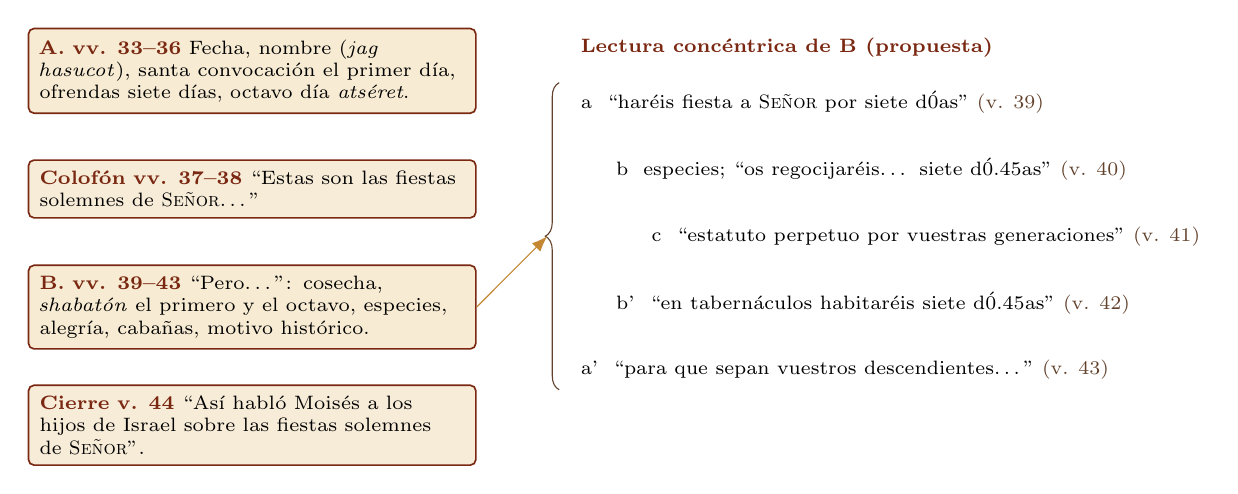
\begin{tikzpicture}[font=\scriptsize,x=1cm,y=1cm]
 \node[caja,text width=5.4cm,anchor=west] (a) at (0,0) {\textbf{\textcolor{tierraroja}{A. vv. 33--36}} Fecha, nombre (\emph{jag hasucot}), santa convocación el primer día, ofrendas siete días, octavo día \emph{atséret}.};
 \node[caja,text width=5.4cm,anchor=west,fill=mostaza!20] (c) at (0,-1.5) {\textbf{\textcolor{tierraroja}{Colofón vv. 37--38}} ``Estas son las fiestas solemnes de \SENOR\ldots''};
 \node[caja,text width=5.4cm,anchor=west] (b) at (0,-3.0) {\textbf{\textcolor{tierraroja}{B. vv. 39--43}} ``Pero\ldots'': cosecha, \emph{shabatón} el primero y el octavo, especies, alegría, cabañas, motivo histórico.};
 \node[caja,text width=5.4cm,anchor=west,fill=mostaza!20] (d) at (0,-4.5) {\textbf{\textcolor{tierraroja}{Cierre v. 44}} ``Así habló Moisés a los hijos de Israel sobre las fiestas solemnes de \SENOR''.};
 \node[anchor=west,text=tierraroja,font=\scriptsize\bfseries] at (6.9,0.3) {Lectura concéntrica de B (propuesta)};
 \foreach \y/\i/\t/\r in {-0.4/0/{a\ \ ``haréis fiesta a \SENOR{} por siete días''}/v. 39, -1.25/0.45/{b\ \ especies; ``os regocijaréis\ldots{} siete días''}/v. 40, -2.1/0.9/{c\ \ ``estatuto perpetuo por vuestras generaciones''}/v. 41, -2.95/0.45/{b'\ \ ``en tabernáculos habitaréis siete días''}/v. 42, -3.8/0/{a'\ \ ``para que sepan vuestros descendientes\ldots''}/v. 43}{
   \node[anchor=west] at (6.9+\i,\y) {\t\ {\color{sepia}(\r)}};}
 \draw[decorate,decoration={brace,amplitude=5pt},sepia] (6.75,-4.05) -- (6.75,-0.15);
 \draw[-{Latex[length=2mm]},mostaza!80!tierraroja] (b.east) -- (6.6,-2.1);
\end{tikzpicture}\par
{\footnotesize\color{sepia}\textit{Figura 7.} Estructura de Lv 23:33--44 y lectura concéntrica de la segunda instrucción. \textit{Nota.} Elaboración propia; la disposición concéntrica es una propuesta de lectura.}
\end{center}

En la segunda instrucción la expresión \heb{שִׁבְעַת יָמִים} (\emph{shivat yamim}, ``siete días'') aparece en cada verso de 39 a 42, y en toda la sección (vv. 33--43) seis veces (conteo hecho sobre el Códice de Leningrado). El ``octavo día'' aparece dos veces (vv. 36, 39). El estribillo de los siete días queda enmarcado por el verbo ``saber'' y por la firma ``Yo \SENOR{} vuestro Dios'', de modo que la fiesta termina en conocimiento de Dios.

\subsection{La alegría como mandato}
Deuteronomio 16 permite comparar las tres fiestas de peregrinación. Para Pésaj y Matsot (16:1--8) no hay verbo de alegría; es memoria del ``pan de aflicción'' (16:3). Para Shavuot hay uno, ``te alegrarás delante de \SENOR'' (16:11). Para Sukkot hay dos, y el segundo es enfático: ``te alegrarás en tus fiestas solemnes'' (16:14) y ``estarás verdaderamente alegre'' (16:15). En todo Levítico el verbo \emph{samaj} aparece una sola vez, en Lv 23:40, dentro de la sección de Sukkot (conteos hechos sobre el Códice de Leningrado). La progresión es literaria y teológica a la vez: el año empieza con la memoria de la esclavitud y termina con la alegría completa.

La alegría tiene destinatarios. Dt 16:14 enumera a ``tu hijo, tu hija, tu siervo, tu sierva, y el levita, el extranjero, el huérfano y la viuda''. Lo que se manda no es un estado de ánimo privado sino una mesa abierta, y por eso puede darse en imperativo: se ordena hacer fiesta con otros ``delante de \SENOR'', no sentir algo.

\subsection{El siete y el octavo}
Sukkot es la fiesta del siete: séptimo mes, siete días, setenta novillos, catorce carneros, noventa y ocho corderos, siete machos cabríos. El octavo día queda fuera de la serie. En la Torá el octavo día marca con frecuencia un comienzo después de un ciclo cumplido: la circuncisión del niño ``de edad de ocho días'' (Gn 17:12; cf. Lv 12:3); la consagración de los sacerdotes, que se completa ``en el día octavo'' (Lv 9:1); la purificación del leproso y del impuro, que termina con una ofrenda el octavo día (Lv 14:10; 15:14); el primogénito del ganado, que se entrega ``al octavo día'' (Éx 22:30 [22:29]); el altar del templo futuro, que funciona ``del octavo día en adelante'' (Ez 43:27). El octavo es el día en que lo preparado durante siete empieza a funcionar.

Ese patrón explica dos desarrollos posteriores. La \emph{Epístola de Bernabé} (ca. 130 e.\,c.) interpreta el octavo día como ``principio de otro mundo'' y lo vincula con el domingo de la resurrección (Bern. 15:8--9; Holmes, 2007); la serie lo lee como el período posterior al Milenio (§7.4). Las dos lecturas coinciden en lo que el texto sí sugiere: que el octavo día no prolonga los siete, sino que es algo distinto.

\subsection{Una fiesta para las naciones}
Sukkot es la fiesta en que la Biblia abre con más claridad el culto de Israel a los extranjeros. Deuteronomio incluye al \heb{גֵּר} (\emph{guer}, extranjero residente) en la alegría (16:14) y en la lectura de la Ley (31:12). Salomón, en la dedicación del templo durante la fiesta, ora por el extranjero ``que no es de tu pueblo Israel'', ``para que todos los pueblos de la tierra conozcan tu nombre'' (1~R 8:41--43). Zacarías termina su libro con las naciones subiendo cada año a celebrar Sukkot (Zac 14:16), y en Juan, durante la misma fiesta, los adversarios se preguntan si Jesús ``se irá a los dispersos entre los griegos, y enseñará a los griegos'' (Jn 7:35). La tradición de los setenta novillos por las setenta naciones (b. Sukká 55b) sigue esa misma línea.

\subsection{De la tienda del desierto a la morada de Dios con los hombres}
Leído en conjunto, el canon muestra una trayectoria. Dios ``hizo habitar'' a Israel en cabañas y, al mismo tiempo, pidió una tienda para habitar él en medio del campamento (Éx 25:8). Cuando la tienda se volvió templo, la dedicación se hizo en Sukkot y la nube llenó la casa (1~R 8:2, 10--11). Los profetas prometieron una morada definitiva (Ez 37:27; 43:7). Juan presenta la encarnación con el verbo de la tienda: el Verbo ``puso su tienda'' entre nosotros, ``y vimos su gloria'' (Jn 1:14), como Israel vio la gloria en la tienda (Éx 40:34). Pablo aplica la promesa de Lv 26:11--12 a la iglesia, ``vosotros sois el templo del Dios viviente'' (2~Co 6:16), y el Apocalipsis cierra con la misma palabra: ``He aquí el tabernáculo de Dios con los hombres, y él morará con ellos'' (Ap 21:3).

\begin{center}
\begin{tikzpicture}[font=\scriptsize,x=1cm,y=1cm]
 \foreach \x/\n/\t/\r/\h in {0/1/{Tienda}/{Éx 25:8; 40:34}/{``habitaré en medio de ellos''}, 2.55/2/{Templo}/{1 R 8:2, 10--11}/{dedicado en Sukkot}, 5.1/3/{Promesa}/{Ez 37:27; Os 12:9}/{``mi tabernáculo'' entre ellos}, 7.65/4/{Encarnación}/{Jn 1:14}/{\grc{ἐσκήνωσεν}}, 10.2/5/{Iglesia}/{2 Co 6:16; Ap 7:15}/{templo del Dios viviente}, 12.75/6/{Consumación}/{Ap 21:3}/{\grc{ἡ σκηνὴ τοῦ θεοῦ}}}{
   \node[caja,text width=2.0cm,align=center,minimum height=1.55cm] (t\n) at (\x,0) {\textbf{\textcolor{tierraroja}{\t}}\\[2pt]{\tiny\color{sepia}\r}\\[1pt]{\tiny\itshape \h}};}
 \foreach \a/\b in {1/2,2/3,3/4,4/5,5/6}{\draw[-{Latex[length=2mm]},mostaza!80!tierraroja,line width=1pt] (t\a) -- (t\b);}
 \draw[sepia,line width=0.6pt] (0,-1.15) -- (12.75,-1.15);
 \foreach \x/\t in {0/{Israel en cabañas (Lv 23:43)}, 3.8/{Abraham en tiendas (He 11:9)}, 7.65/{el cuerpo, ``tienda'' (2 Co 5:1; 2 P 1:14)}, 12.0/{``casa no hecha de manos''}}{
   \fill[mostaza] (\x,-1.15) circle (2pt);
   \node[below=3pt,font=\tiny,text=sepia,text width=2.6cm,align=center] at (\x,-1.15) {\t};}
 \node[anchor=east,font=\tiny\itshape,text=tierraroja] at (-1.2,0) {Dios mora};
 \node[anchor=east,font=\tiny\itshape,text=tierraroja] at (-1.2,-1.15) {el hombre mora};
\end{tikzpicture}\par
{\footnotesize\color{sepia}\textit{Figura 8.} Trayectoria canónica de la tienda: dos líneas que se encuentran en Ap 21:3. \textit{Nota.} Elaboración propia.}
\end{center}

La figura muestra dos líneas paralelas. Arriba, la morada de Dios con su pueblo; abajo, la morada del hombre, siempre provisoria: Abraham en tiendas, Israel en cabañas, el creyente en un cuerpo que Pablo llama ``tienda''. Sukkot pone las dos líneas en la misma semana, con Israel en cabañas y Dios en su santuario en medio de ellos, y Ap 21:3 es el punto donde la tienda de Dios y la de los hombres se vuelven una sola.

%===================================================================
\section{Memorial, figura y esperanza: la lectura de la serie}

La serie lee cada fiesta como memorial de un hito de la historia de Israel y figura de una etapa del plan de salvación. Para Sukkot, su tesis se resume en cinco pasos.

\subsection{Memorial del desierto y figura de la tierra}
La relación de Sukkot con la historia de Israel es doble. Un nexo está en la letra del mandato, ``para que sepan vuestros descendientes, que en cabañas hice yo habitar'' a Israel (Lv 23:43); el otro se deduce de la secuencia del mes séptimo. Si Trompetas recuerda la caída de Jericó al son de las trompetas, y Expiación el fin del juicio del desierto y el perdón antes de entrar, Cabañas señala el momento en que Israel se establece como reino en la tierra que Dios había prometido a Abraham, aunque eso fuera entonces solo una situación temporal, como explica Hebreos. De ahí la conclusión doble de la serie: Sukkot es, en la historia de Israel, conmemoración de la travesía por el desierto y símbolo de la toma de posesión de la Tierra Prometida.

La serie da tres razones para observar la fiesta: su carácter perpetuo (Lv 23:41), su sentido histórico (Lv 23:42--43) y su perspectiva simbólica, que le otorga vigencia (Col 2:16--17). Añade un argumento práctico, que la Iglesia apostólica la conocía, como muestra Juan 7.

\begin{nota}[Precisión]
El vínculo con el desierto está en el texto (Lv 23:43). El vínculo con la entrada en Canaán es lectura tipológica de la serie. Tiene apoyos indirectos: la fiesta supone la cosecha de la tierra ya poseída (Lv 23:39; Dt 16:13--15); Nehemías la relaciona con ``los días de Josué hijo de Nun'' (Neh 8:17); y el primer Sukkot posible después del éxodo, con cosecha propia, solo podía celebrarse en la tierra. Pero el cruce del Jordán ocurrió ``el día diez del mes primero'' y la primera Pascua en Gilgal el 14 (Jos 4:19; 5:10), en primavera, no en el mes séptimo. La correspondencia es de sentido (desierto $\rightarrow$ tierra), no de calendario. Sobre la autoría de Hebreos, que la serie atribuye a Pablo, véase la nota de §8.4.
\end{nota}

\subsection{Para la Iglesia: el Reino milenial}
En la lectura de la serie, Trompetas y Expiación simbolizan el retorno del Señor Jesús: la resurrección de los muertos en Cristo, la transformación de los vivos, el fin del juicio a la Iglesia y el prendimiento de Satanás (Ap 20:1--3). Todo eso es el preludio del establecimiento del Reino milenial de Dios con sus santos. Sukkot simboliza ese Reino: ``Bienaventurado y santo el que tiene parte en la primera resurrección; la segunda muerte no tiene potestad sobre éstos, sino que serán sacerdotes de Dios y de Cristo, y reinarán con él mil años'' (Ap 20:6). Así como Israel entró en su tierra precedido por trompetas y después del juicio del desierto, la Iglesia entrará en el Reino prometido (Jn 14:1--3), precedida por la trompeta (1~Ts 4:16--17) y no antes de que concluya el juicio ya presente entre sus miembros (1~P 4:17), y pondrá sus pies en la Tierra Prometida (Zac 14:4--5).

\subsection{La cabaña: lo pasajero}
La cabaña es el elemento central. La morada endeble que se habita durante la fiesta representa, en cierto modo, la levedad de la propia existencia. Reunir a toda la comunidad en un lugar, dejando viviendas, trabajos y complicaciones, simboliza la esperanza de lo que será la existencia en el tiempo del Milenio. De allí sale la conclusión sobre la que descansa todo lo demás: lo temporal del habitar en cabañas durante los días de la fiesta indica con claridad que el Milenio no es la eternidad, porque todavía falta cerrar el ciclo de la existencia de la humanidad alejada de Dios.

La filología apoya la primera parte del argumento. La \emph{sucá} es, en todo el Antiguo Testamento, una construcción provisoria (Is 1:8; Jon 4:5; Job 27:18); la Misná fija que durante siete días la cabaña es ``fija'' y la casa ``provisoria'' (Misná Sukká 2:9), con una inversión que dura solo la semana; y el Nuevo Testamento usa la tienda como imagen de lo que se deshace (2~Co 5:1; 2~P 1:13--14).

\subsection{El Octavo día: después del Milenio}
La serie recuerda que en la segunda venida solo resucitan quienes forman parte del gobierno de Dios, porque ``los otros muertos no volvieron a vivir hasta que se cumplieron mil años'' (Ap 20:5). Después del Milenio vienen otros sucesos:

\begin{cita}Cuando los mil años se cumplan, Satanás será suelto de su prisión, y saldrá a engañar a las naciones que están en los cuatro ángulos de la tierra, a Gog y a Magog, a fin de reunirlos para la batalla; el número de los cuales es como la arena del mar.\fuente{(Ap 20:7--8)}\end{cita}

\begin{cita}Y vi un gran trono blanco y al que estaba sentado en él, de delante del cual huyeron la tierra y el cielo, y ningún lugar se encontró para ellos. Y vi a los muertos, grandes y pequeños, de pie ante Dios; y los libros fueron abiertos, y otro libro fue abierto, el cual es el libro de la vida; y fueron juzgados los muertos por las cosas que estaban escritas en los libros, según sus obras.\fuente{(Ap 20:11--12)}\end{cita}

Este relato permite comprender el significado simbólico del octavo día de la fiesta: el tiempo después del Milenio, en que se desarrollarán los acontecimientos de Ap 20:7--15, que culminan con el gran juicio final. La serie lo une con Pablo, ``Luego el fin, cuando entregue el reino al Dios y Padre\ldots{} para que Dios sea todo en todos'' (1~Co 15:24, 28), y añade una regla práctica: aunque la orden es habitar siete días en cabañas, se permanece en ellas el octavo por la condición de sábado que el Reglamento del Culto confiere a ese día.

\begin{center}
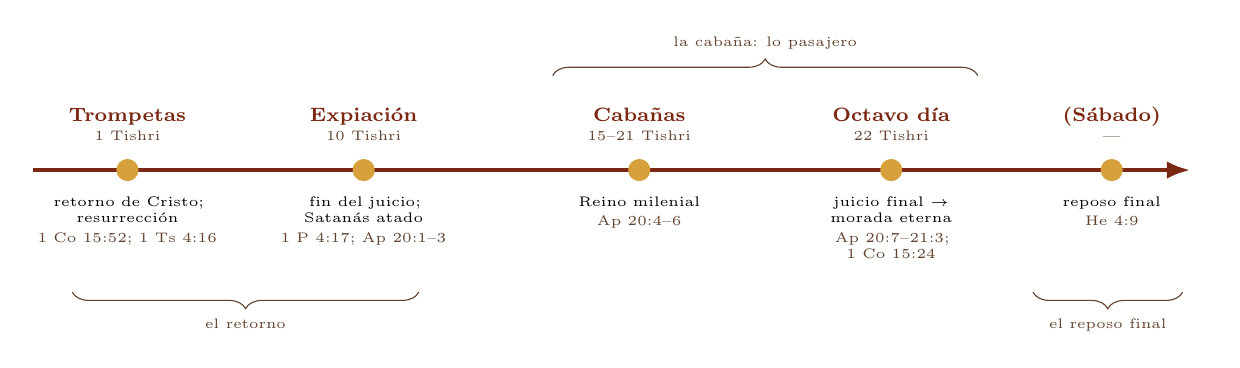
\begin{tikzpicture}[font=\scriptsize,x=1cm,y=1cm]
 \draw[line width=1.6pt,tierraroja,-{Latex[length=3mm]}] (-0.3,0) -- (14.4,0);
 \foreach \x/\f/\d/\e/\r in {0.9/{Trompetas}/{1 Tishri}/{retorno de Cristo; resurrección}/{1 Co 15:52; 1 Ts 4:16}, 3.9/{Expiación}/{10 Tishri}/{fin del juicio; Satanás atado}/{1 P 4:17; Ap 20:1--3}, 7.4/{Cabañas}/{15--21 Tishri}/{Reino milenial}/{Ap 20:4--6}, 10.6/{Octavo día}/{22 Tishri}/{juicio final $\rightarrow$ morada eterna}/{Ap 20:7--21:3; 1 Co 15:24}, 13.4/{(Sábado)}/{---}/{reposo final}/{He 4:9}}{
   \fill[mostaza] (\x,0) circle (4pt);
   \node[above=7pt,font=\scriptsize\bfseries,text=tierraroja,align=center] at (\x,0) {\f\\[-1pt]{\tiny\mdseries\color{sepia}\d}};
   \node[below=6pt,text width=2.3cm,align=center,font=\tiny] at (\x,0) {\e\\[1pt]{\color{sepia}\r}};}
 \draw[decorate,decoration={brace,amplitude=6pt},sepia] (6.3,1.2) -- (11.7,1.2) node[midway,above=6pt,font=\tiny,text=sepia]{la cabaña: lo pasajero};
 \draw[decorate,decoration={brace,amplitude=6pt,mirror},sepia] (0.2,-1.55) -- (4.6,-1.55) node[midway,below=6pt,font=\tiny,text=sepia]{el retorno};
 \draw[decorate,decoration={brace,amplitude=6pt,mirror},sepia] (12.4,-1.55) -- (14.3,-1.55) node[midway,below=6pt,font=\tiny,text=sepia]{el reposo final};
\end{tikzpicture}\par
{\footnotesize\color{sepia}\textit{Figura 9.} La secuencia final del ciclo como línea de tiempo profética, según la lectura de la serie. \textit{Nota.} Elaboración propia. El Sábado como figura del reposo final (He 4:9) es también lectura de la serie. El Octavo día desemboca en la morada eterna (Ap 21:1--3; §7.6).}
\end{center}

\subsection{Las dos suposiciones que la serie refuta}
La serie cierra su lectura de la fiesta con dos objeciones que considera erróneas.

\textbf{Primera: durante el Milenio será el tiempo de celebrar esta fiesta, no ahora.} Esta postura se apoya en Zac 14:16. La serie responde con una pregunta al texto: ¿quiénes subirán de año en año a Jerusalén? ``Todos los que sobrevivieren de las naciones que vinieron contra Jerusalén''. El versículo no inaugura la fiesta en el futuro; describe a los pueblos que la aprenderán después de ser sometidos al gobierno de Dios, compuesto por Jesús y sus santos. El Milenio extiende a las naciones una fiesta que el pueblo de Dios ya celebra por estatuto perpetuo (Lv 23:41), como la celebró Jesús (Jn 7). La pregunta que queda es pastoral: ¿en qué frente quiere estar cada uno?

\textbf{Segunda: Sukkot es símbolo de la eternidad.} La serie responde desde el elemento central de la fiesta: la cabaña no puede simbolizar la eternidad, porque su sentido es lo pasajero, la levedad de la existencia. Solo después del Milenio y de los acontecimientos del Octavo día, quienes vivan esos momentos podrán conocer lo que será la eternidad. La lectura que adopta este capítulo (§7.6) mantiene el argumento: la cabaña no es la eternidad, y el Octavo día, que ya no forma parte de los ``siete días'' en cabañas (Lv 23:42), es el umbral que lleva a ella.

El argumento se sostiene en el propio texto. En Zac 14:16--19 la fiesta va unida a amenazas de sequía y de plaga para quien no suba, lo que supone un mundo donde todavía cabe la desobediencia, algo que no corresponde a Ap 21:4 (``ya no habrá muerte, ni habrá más llanto''); y la cabaña, por definición, es provisoria. La serie separa así la figura (la cabaña) de la realidad final (la ``casa no hecha de manos'', 2~Co 5:1; la ciudad ``con fundamentos'', He 11:10).

\subsection{El Octavo día: del juicio final a la morada eterna}
La lectura de la serie y mi presentación anterior coinciden en los siete días y acentúan dos aspectos distintos del octavo. La serie lee el octavo día como el tiempo posterior al Milenio, con la suelta de Satanás, Gog y Magog y el juicio del gran trono blanco (Ap 20:7--15), y niega que la cabaña simbolice la eternidad. En mi presentación anterior sobre Sukkot escribí, entre los ``aspectos proféticos'', que los siete días representan el reino milenial del Señor con sus santos (Ap 20:4; Zac 14:16) y que el octavo día ``representaría la eternidad, cuando el Padre mismo establece su tabernáculo entre los hombres'' (Ap 21:3). Las dos afirmaciones caben en una sola lectura, por tres razones:
\begin{itemize}
\item \textbf{La cabaña termina con los siete días.} Para ambas lecturas, los siete días en cabañas son el Milenio y la cabaña es lo provisorio. Según Lv 23:42, se habita en cabañas ``siete días'', de modo que el octavo ya no es un día de cabaña, y atribuirle la entrada en la eternidad no contradice que la cabaña no sea la eternidad.
\item \textbf{Ap 20 y 21 son una secuencia continua.} El juicio del gran trono blanco (20:11--15) desemboca sin interrupción en ``un cielo nuevo y una tierra nueva'' y en ``el tabernáculo de Dios con los hombres'' (21:1--3). Pablo resume el mismo paso: ``Luego el fin, cuando entregue el reino al Dios y Padre\ldots{} para que Dios sea todo en todos'' (1~Co 15:24, 28). ``El fin'' incluye el último juicio y la entrega del reino al Padre.
\item \textbf{La filología del octavo día es la de un umbral.} \emph{Atséret} viene de ``detener, retener'' y designa la asamblea de clausura; la LXX la llama \grc{ἐξόδιον}, ``salida'' (§4.3). Un día de clausura cierra un ciclo y abre lo que sigue.
\end{itemize}

\begin{tcolorbox}[enhanced,unbreakable,colback=papiro,colframe=tierraroja,boxrule=1pt,arc=3pt,title={\textbf{Lectura de la serie: el Octavo día}},coltitle=papiro,colbacktitle=tierraroja]
\small Los \textbf{siete días} en cabañas figuran el \textbf{Reino milenial} de Cristo con sus santos (Ap 20:4--6; Zac 14:16); la cabaña indica que esa etapa es todavía provisoria y no es la eternidad. El \textbf{Octavo día} figura el tiempo \textbf{posterior al Milenio}: la última rebelión y el juicio final ante el gran trono blanco (Ap 20:7--15), que \textbf{desemboca en la morada eterna} de Dios con los hombres: ``He aquí el tabernáculo de Dios con los hombres, y él morará con ellos'' (Ap 21:1--3), cuando Dios sea ``todo en todos'' (1~Co 15:24--28). \emph{Atséret} (``clausura, retención'') y la LXX \grc{ἐξόδιον} (``salida'') apoyan leerlo como umbral. El \textbf{Sábado} sigue siendo figura del reposo final que queda para el pueblo de Dios (He 4:9). Esta lectura integra el juicio posterior al Milenio (Ap 20:7--15) y ``luego el fin'' (1~Co 15:24) con mi presentación anterior (``el Padre mismo establece su tabernáculo entre los hombres'', Ap 21:3), sin contradicción: la cabaña no es la eternidad, y el octavo día no es una cabaña.
\end{tcolorbox}

\subsection{Precisiones sobre la lectura de la serie}
\begin{nota}[Precisión]
(1) \textbf{Dos acentos en el Octavo día.} El Octavo día puede leerse también, con el nombre de ``el Último Gran Día'' tomado de Jn 7:37, como la segunda resurrección de Ap 20:5, 11--12 y Ez 37, con una oportunidad de salvación para quienes nunca conocieron el evangelio. La serie pone el acento en el juicio final y en ``luego el fin''. Las dos lecturas coinciden en ubicar el Octavo día después del Milenio; la lectura adoptada (§7.6) recoge el juicio y su desenlace en la morada eterna.\par
(2) \textbf{``El último y gran día''.} Jn 7:37 no dice si se trata del séptimo día (el de las siete vueltas con el sauce) o del octavo (\emph{atséret}); la libación del agua duraba siete días (Misná Sukká 4:1). Los comentarios se dividen (Brown, 1966; Keener, 2003). El nombre ``Último Gran Día'' para el octavo es una designación posterior, no del texto de Levítico.\par
(3) \textbf{``Luego el fin''.} En 1~Co 15:24 \grc{εἶτα τὸ τέλος} se traduce ``luego el fin''. Algunos intérpretes leyeron \grc{τὸ τέλος} como ``el resto'' (un tercer grupo de resucitados) y vieron allí un intervalo milenial; Fee (1987) lo rechaza y lee ``el fin''. El intervalo entre la venida de Cristo y ``el fin'' es claro en el texto (``luego\ldots{} luego''); su duración no la da Pablo, sino Ap 20.\par
(4) \textbf{Abraham ``en cabañas''.} La serie lee He 11:9 como ``habitando en cabañas''; el griego dice \grc{ἐν σκηναῖς}, ``en tiendas''. La lectura es legítima porque la LXX usa \grc{σκηναί} también para las \emph{sucot} de Lv 23. Los Jubileos (16:20--31) ya hacían de Abraham el primero en celebrar Sukkot.
\end{nota}

\begin{center}\begin{minipage}{\linewidth}\centering\small\renewcommand{\arraystretch}{1.22}
\begin{tabular}{@{}L{3.6cm}L{3.0cm}L{7.8cm}@{}}
\toprule
\textbf{Hito de Israel} & \textbf{Fiesta} & \textbf{Nuevo Pacto (lectura de la serie)} \\ \midrule
Caída de Jericó al son de trompetas & Trompetas (1 Tishri) & Retorno de Cristo a la final trompeta (1~Co 15:51--52; 1~Ts 4:16; Ap 11:15) \\
Fin del juicio del desierto & Expiación (10 Tishri) & Fin del juicio a la casa de Dios (1~P 4:17); Satanás atado (Ap 20:1--3) \\
Desierto en cabañas; entrada a Canaán & Cabañas (15--21 Tishri) & Reino milenial; la cabaña = lo pasajero; el Milenio no es la eternidad \\
(después) & Octavo día (22 Tishri) & Después del Milenio: Gog y Magog, gran trono blanco (Ap 20:7--15), que desemboca en la morada eterna (Ap 21:1--3); ``luego el fin'' (1~Co 15:24--28) \\
\bottomrule
\end{tabular}\par
{\footnotesize\color{sepia}\textit{Tabla 4.} La secuencia del mes séptimo en la lectura de la serie. \textit{Nota.} Elaboración propia.}
\end{minipage}\end{center}

%===================================================================
\section{Sukkot en Jesús y los apóstoles}

\subsection{Juan 7--8: el agua y la luz}
Juan sitúa en Sukkot la sección más larga de su evangelio dedicada a una fiesta (Jn 7:1--10:21). ``Estaba cerca la fiesta de los judíos, la de los tabernáculos'' (7:2). Los hermanos de Jesús le piden que suba y se manifieste al mundo; él responde que su tiempo no ha llegado (7:6--8) y sube después, en secreto (7:10). ``A la mitad de la fiesta'' (\grc{τῆς ἑορτῆς μεσούσης}) enseña en el templo (7:14), y en el día culminante hace su proclamación:

\begin{cita}En el último y gran día de la fiesta, Jesús se puso en pie y alzó la voz, diciendo: Si alguno tiene sed, venga a mí y beba. El que cree en mí, como dice la Escritura, de su interior correrán ríos de agua viva. Esto dijo del Espíritu que habían de recibir los que creyesen en él; pues aún no había venido el Espíritu Santo, porque Jesús no había sido aún glorificado.\fuente{(Jn 7:37--39)}\end{cita}

\begin{cita}Otra vez Jesús les habló, diciendo: Yo soy la luz del mundo; el que me sigue, no andará en tinieblas, sino que tendrá la luz de la vida.\fuente{(Jn 8:12)}\end{cita}

El trasfondo es el culto descrito en §3.4. Durante siete mañanas la ciudad había visto el agua de Siloé derramada sobre el altar, entre cantos de Is 12:3, y durante las noches los candelabros del atrio de las mujeres iluminaban Jerusalén. Jesús toma las dos imágenes y las aplica a sí mismo. Juan sitúa la segunda declaración ``en el lugar de las ofrendas'' (8:20), en el tesoro, que la Misná ubica en ese mismo atrio; y el capítulo siguiente retoma el agua y la luz, cuando Jesús, que dice ``luz soy del mundo'' (9:5), envía al ciego a lavarse ``en el estanque de Siloé (que traducido es, Enviado)'' (9:7), el estanque del que se sacaba el agua de la fiesta (Keener, 2003).

\begin{center}
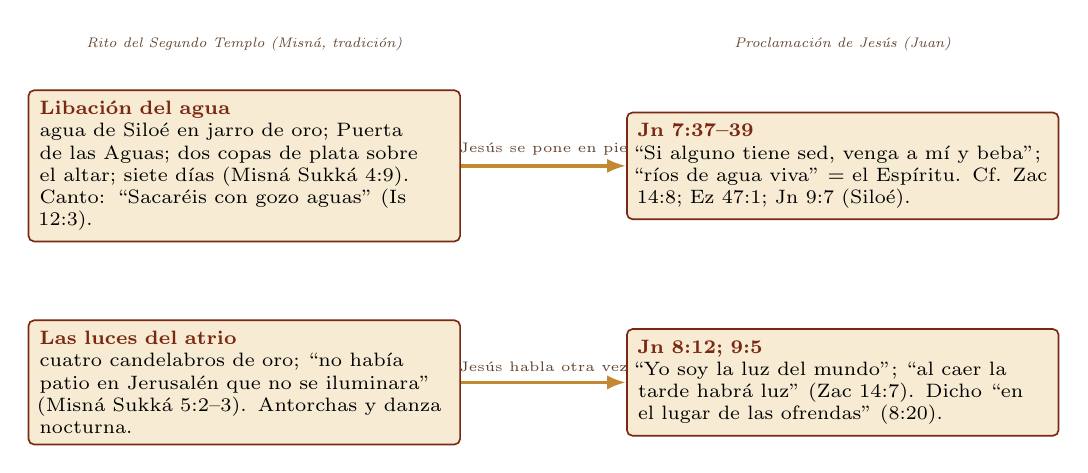
\begin{tikzpicture}[font=\scriptsize,x=1cm,y=1cm]
 \node[caja,text width=5.2cm] (r1) at (0,0) {\textbf{\textcolor{tierraroja}{Libación del agua}}\\ agua de Siloé en jarro de oro; Puerta de las Aguas; dos copas de plata sobre el altar; siete días (Misná Sukká 4:9). Canto: ``Sacaréis con gozo aguas'' (Is 12:3).};
 \node[caja,text width=5.2cm] (j1) at (7.6,0) {\textbf{\textcolor{tierraroja}{Jn 7:37--39}}\\ ``Si alguno tiene sed, venga a mí y beba''; ``ríos de agua viva'' = el Espíritu. Cf. Zac 14:8; Ez 47:1; Jn 9:7 (Siloé).};
 \node[caja,text width=5.2cm] (r2) at (0,-2.75) {\textbf{\textcolor{tierraroja}{Las luces del atrio}}\\ cuatro candelabros de oro; ``no había patio en Jerusalén que no se iluminara'' (Misná Sukká 5:2--3). Antorchas y danza nocturna.};
 \node[caja,text width=5.2cm] (j2) at (7.6,-2.75) {\textbf{\textcolor{tierraroja}{Jn 8:12; 9:5}}\\ ``Yo soy la luz del mundo''; ``al caer la tarde habrá luz'' (Zac 14:7). Dicho ``en el lugar de las ofrendas'' (8:20).};
 \draw[-{Latex[length=2.4mm]},mostaza!80!tierraroja,line width=1.2pt] (r1) -- node[above,font=\tiny,text=sepia]{Jesús se pone en pie} (j1);
 \draw[-{Latex[length=2.4mm]},mostaza!80!tierraroja,line width=1.2pt] (r2) -- node[above,font=\tiny,text=sepia]{Jesús habla otra vez} (j2);
 \node[text=sepia,font=\tiny\itshape,align=center] at (0,1.55) {Rito del Segundo Templo (Misná, tradición)};
 \node[text=sepia,font=\tiny\itshape,align=center] at (7.6,1.55) {Proclamación de Jesús (Juan)};
\end{tikzpicture}\par
{\footnotesize\color{sepia}\textit{Figura 10.} El agua y la luz: del rito de Sukkot a las palabras de Jesús en Juan 7--8. \textit{Nota.} Elaboración propia. El rito se conoce por la Misná, posterior al templo.}
\end{center}

La lógica de Juan es la del cumplimiento: lo que el templo hacía con agua de Siloé y luz de lámparas se cumple en una persona. El agua que Ezequiel vio salir del santuario (Ez 47:1) y Zacarías salir de Jerusalén (Zac 14:8) sale ahora de Cristo hacia los que creen. Juan añade una nota de tiempo, pues el Espíritu aún no había venido ``porque Jesús no había sido aún glorificado'' (7:39); la promesa de Sukkot espera la cruz, la resurrección y Pentecostés.

\subsection{``Y habitó entre nosotros''}
El prólogo de Juan describe la encarnación con el vocabulario de la tienda: \grc{Καὶ ὁ λόγος σὰρξ ἐγένετο καὶ ἐσκήνωσεν ἐν ἡμῖν}, ``Y aquel Verbo fue hecho carne, y habitó entre nosotros (y vimos su gloria\ldots)'' (Jn 1:14). La frase reúne tres elementos del Éxodo: la tienda (\grc{σκηνή}), la gloria que la llena (Éx 40:34) y Dios que habita ``en medio'' de su pueblo (Éx 25:8). Coloe (2001) muestra que Juan desarrolla esta teología del templo a lo largo del evangelio; el cuerpo de Jesús es el templo (2:19--21), y la fiesta de las cabañas es una de las ocasiones en que esa sustitución se hace visible.

\begin{nota}[Precisión]
Algunos autores deducen de Jn 1:14 que Jesús nació durante Sukkot. Juan no lo dice, y los evangelios no dan la fecha del nacimiento. El verbo \grc{ἐσκήνωσεν} remite al tabernáculo del desierto, no a la fecha de la fiesta. Es una deducción posible dentro de lecturas tipológicas, no una enseñanza del texto.
\end{nota}

\subsection{Las tres enramadas de la transfiguración}
Pedro, al ver a Jesús transfigurado con Moisés y Elías, propone: ``Señor, bueno es para nosotros que estemos aquí; si quieres, hagamos aquí tres enramadas: una para ti, otra para Moisés, y otra para Elías'' (Mt 17:4). Lucas añade que hablaban ``de su partida'', literalmente ``de su éxodo'' (\grc{τὴν ἔξοδον αὐτοῦ}, Lc 9:31). La serie ve en la propuesta de Pedro una comprensión de la relación entre las tiendas y el Reino de Dios. Algunos estudiosos han relacionado la escena con Sukkot por las tiendas, la gloria y la fecha ``seis días después'' (Mt 17:1); Daniélou (1956) recoge esa lectura. El texto, sin embargo, corrige a Pedro: la voz del cielo no aprueba las tiendas, sino que manda oír al Hijo (17:5). Las enramadas querían fijar la gloria en un lugar, cuando el camino pasaba todavía por el éxodo de Jerusalén.

\subsection{Palmas, tiendas y extranjeros}
\textbf{Jn 12:13.} En la entrada a Jerusalén la multitud ``tomó ramas de palmera'' y clamó ``¡Hosanna!'' con palabras del Sal 118:25--26. El gesto y el salmo pertenecen a Sukkot, pero la escena ocurre seis días antes de la Pascua (12:1), y no hay que leerla como un Sukkot fuera de fecha: las palmas eran ya signo nacional de victoria y de bienvenida al rey (1~Mac 13:51; 2~Mac 10:7), y el Sal 118 se cantaba en el Hallel de todas las fiestas de peregrinación.

\textbf{Ap 7:9--17.} Juan ve ``una gran multitud\ldots{} de todas naciones y tribus y pueblos y lenguas'', ``vestidos de ropas blancas, y con palmas en las manos'' (7:9). El que está en el trono ``extenderá su tabernáculo sobre ellos'' (\grc{σκηνώσει}, 7:15); ``ya no tendrán hambre ni sed'', y el Cordero ``los guiará a fuentes de aguas de vida'' (7:16--17; cf. Is 49:10). Palmas, tienda, agua y naciones son los temas de Sukkot. Ulfgard (1989) estudió el pasaje como una lectura escatológica de la fiesta, y Bauckham (1993) muestra cómo el Apocalipsis reúne imágenes de cosecha y de fiesta para describir la reunión de las naciones.

\textbf{He 11:9--10, 13--16.} Abraham habitó ``como extranjero en la tierra prometida como en tierra ajena, morando en tiendas con Isaac y Jacob\ldots{} porque esperaba la ciudad que tiene fundamentos, cuyo arquitecto y constructor es Dios''. Los patriarcas confesaron ``que eran extranjeros y peregrinos sobre la tierra'' y buscaban ``una patria\ldots{} mejor, esto es, celestial''. Es el comentario neotestamentario más cercano al sentido de la cabaña: la tienda no es el destino sino la manera de vivir mientras se espera.

\begin{nota}[Precisión]
La serie atribuye Hebreos al apóstol Pablo. La autoría de Hebreos es discutida desde la Antigüedad: Orígenes dijo que solo Dios sabe quién la escribió, y los comentarios modernos la consideran anónima, de un autor del círculo paulino (Attridge, 1989; Lane, 1991). El argumento de la serie no depende de la autoría: depende de que Hebreos lea la vida en tiendas como espera de la ciudad.
\end{nota}

\subsection{Pablo: la tienda del cuerpo}
Pablo, ``hacedor de tiendas'' (Hch 18:3), describe el cuerpo mortal con la imagen de la tienda: ``si nuestra morada terrestre, este tabernáculo, se deshiciere, tenemos de Dios un edificio, una casa no hecha de manos, eterna, en los cielos''; ``los que estamos en este tabernáculo gemimos con angustia; porque no quisiéramos ser desnudados, sino revestidos, para que lo mortal sea absorbido por la vida'' (2~Co 5:1, 4). Pedro usa la misma imagen ante su muerte (2~P 1:13--14). Aquí está entera la teología de la cabaña: el creyente vive en algo provisorio y espera lo definitivo, que viene de Dios. La resurrección de 1~Co 15 es el paso de la tienda a la casa, ``es necesario que esto corruptible se vista de incorrupción'' (15:53).

Pablo no menciona Sukkot por nombre. La serie apoya la vigencia de las fiestas en Col 2:16--17: ``Por tanto, nadie os juzgue en comida o en bebida, o en cuanto a días de fiesta, luna nueva o días de reposo, todo lo cual es sombra de lo que ha de venir; pero el cuerpo es de Cristo'', y lee la ``sombra de lo que ha de venir'' como figura todavía abierta hacia el futuro y, por tanto, vigente. Otros comentaristas entienden que la sombra ya encontró su cuerpo en Cristo y que Pablo protege a los creyentes de quienes los juzgaban por observar o no observar esos días (Dunn, 1996). El texto admite discutir si la observancia es obligatoria; lo que no admite es despreciar a quien la guarda ni a quien no la guarda.

%===================================================================
\section{Sukkot en la tradición judía}

La práctica judía actual conserva los rasgos bíblicos y los desarrolla con normas y costumbres de épocas diversas, que aquí se exponen como tradición.

\begin{itemize}
\item \textbf{La sucá y las cuatro especies.} Se come y, si es posible, se duerme en la cabaña durante siete días, con las normas de la Misná (§3.2). Cada día, salvo en sábado, se toman el lulav, el mirto, el sauce y el etrog, se pronuncia una bendición y se agitan hacia los cuatro puntos cardinales, arriba y abajo, durante el Hallel (Misná Sukká 3).
\item \textbf{Hoshanot y Hoshaná Rabá.} Cada día se da una vuelta alrededor del atril de la sinagoga con las especies, recitando súplicas que repiten \emph{hoshá na}; el séptimo día, siete vueltas, como en el altar (Misná Sukká 4:5). En las sinagogas, las vueltas (\emph{hoshanot}) se dan alrededor de la \emph{bimá}, con el rollo de la Torá sacado del arca. En Hoshaná Rabá se dan siete vueltas y se golpean ramas de sauce; se entiende que ese día se pone el sello final al juicio iniciado en Rosh haShaná, y hay costumbre de leer Deuteronomio y estudiar toda la noche. Estas costumbres son medievales, y la vigilia de estudio es de origen cabalístico. En mi presentación anterior las recogí como tradiciones, junto con la \emph{Simjat Beit haShoevá}, Shemini Atséret y Simjat Torá.
\item \textbf{Lecturas.} Zac 14 se lee como \emph{haftará} del primer día y 1~R 8 en el segundo (b. Meguilá 31a); en el sábado de la fiesta se lee el Eclesiastés, costumbre posterior que pone el libro de la vanidad en la semana de la cabaña.
\item \textbf{Ushpizin.} La costumbre de ``invitar'' cada noche a uno de los patriarcas (Abraham, Isaac, Jacob, Moisés, Aarón, José, David) a la cabaña procede de la Cábala (Zóhar, s.~XIII).
\item \textbf{Shemini Atséret.} El Talmud lo considera una fiesta por derecho propio, no un apéndice de Sukkot (b. Sukká 47a). En él comienza la mención de la lluvia en la oración (Misná Taanit 1:1), con la súplica por la lluvia (\emph{Tefilat Guéshem}). Rashi lo explica con la parábola del rey que retiene a sus hijos un día más (§4.3).
\item \textbf{Simjat Torá.} La fiesta de la ``alegría de la Torá'', que cierra y recomienza la lectura anual del Pentateuco, es una creación medieval, que depende del ciclo babilónico de lectura en un año. En la diáspora cae en el segundo día de Shemini Atséret; en Israel, el mismo día.
\item \textbf{La esperanza.} En la bendición después de las comidas de la fiesta se pide: ``El Misericordioso levante para nosotros la sucá de David caída'' (Am 9:11). El Talmud imagina que en el mundo venidero Dios hará para los justos una cabaña con la piel del Leviatán (b. Bava Batra 75a). Son imágenes de la tradición, no doctrina bíblica, pero muestran que la lectura judía también proyecta la cabaña hacia la era mesiánica.
\end{itemize}

%===================================================================
\section{Discusión de interpretaciones}

¿Qué representa Sukkot en el plan de Dios? Las respuestas dependen sobre todo de dos decisiones previas, cómo se lee el Milenio de Ap 20 y qué se hace con la imagen de la tienda en Ap 21:3.

\begin{center}\small\renewcommand{\arraystretch}{1.22}
\begin{tabular}{@{}L{3.0cm}L{5.2cm}L{3.2cm}L{3.0cm}@{}}
\toprule
\textbf{Postura} & \textbf{Lectura de Sukkot} & \textbf{Textos clave} & \textbf{Autores} \\ \midrule
Milenial (lectura de la serie) & Cabañas = Reino milenial; la cabaña indica que no es la eternidad; Octavo día = después del Milenio: juicio final que desemboca en la morada eterna (Ap 20:7--21:3) & Lv 23:42; Zac 14:16; Ap 20; 1~Co 15:24 & la serie \\
Milenarismo patrístico & El verdadero Sukkot en el séptimo milenio, con cuerpos resucitados; el octavo, paso a la eternidad & Lv 23:39--43; Ap 20 & Metodio de Olimpo, \emph{Banquete} 9 (en Daniélou, 1956) \\
Premilenarismo con correspondencia de fiestas & Cabañas = Reino de Cristo en la tierra; Trompetas = arrebatamiento & Zac 14; Ez 37:26--28; Ap 21:3 & Chumney (1994); Baker (2013) \\
Premilenarismo histórico & Ap 20 es un reino futuro, sin correspondencia sistemática con las fiestas & Ap 20:1--6 & Ladd (1972) \\
Amilenarismo / cumplimiento cristológico & Sukkot se cumple en la encarnación (Jn 1:14) y en el Espíritu (Jn 7:39), y se consuma en la morada eterna (Ap 7:15; 21:3) & Jn 1:14; 7:37--39; Ap 21:3 & Hoekema (1979); Beale (1999); Coloe (2001) \\
Lectura judía & Fiesta de la cosecha y del desierto; en la era mesiánica, fiesta de las naciones y sucá de David restaurada & Zac 14; Am 9:11 & Misná; Talmud; Rubenstein (1995) \\
\bottomrule
\end{tabular}\par
{\footnotesize\color{sepia}\textit{Tabla 5.} Lecturas de Sukkot. \textit{Nota.} Elaboración propia.}
\end{center}

Las posturas coinciden en más de lo que parece. Todas reconocen el carácter conmemorativo (Lv 23:43), la alegría de la cosecha, la apertura a las naciones (Zac 14) y la relación con la morada de Dios; las diferencias están en la cronología del cumplimiento.

La lectura de la serie tiene dos puntos fuertes. El primero es la coherencia con el símbolo central, pues la cabaña es en toda la Biblia lo provisorio, y una fiesta de cabañas difícilmente representa la condición definitiva. El segundo es el contexto de Zac 14:16--19, que describe un mundo donde todavía hay naciones que podrían no subir y castigos posibles, algo que no corresponde a la nueva creación de Ap 21:4. Se suma un argumento estructural: la Torá distingue los siete días del octavo, y la serie da contenido a esa distinción.

La objeción más seria viene de Ap 21:3, que describe la eternidad con la palabra de la fiesta, ``He aquí el tabernáculo de Dios con los hombres''; los amilenaristas y muchos premilenaristas ven allí la consumación de Sukkot (Beale, 1999). Una observación del propio texto ayuda a ordenar el debate. En Ap 21:3 la tienda es \emph{de Dios} (\grc{ἡ σκηνὴ τοῦ θεοῦ}), no del hombre: el hombre ya no vive en cabaña provisoria, y es Dios quien ``pone su tienda'' con ellos. La cabaña humana puede entonces representar lo pasajero, como sostiene la serie, mientras la tienda divina, la presencia que mora, alcanza su forma final; las dos líneas de la Figura 8 se encuentran en ese verso. La lectura de la serie (§7.6) da a Ap 21:3 su lugar al final del Octavo día, de modo que la consumación no está en la cabaña de los siete días sino en la morada eterna a la que desemboca el juicio final.

%===================================================================
\section{Síntesis}

\begin{tcolorbox}[enhanced,unbreakable,colback=papiro,colframe=tierraroja,boxrule=1pt,arc=3pt,title={\textbf{Sukkot y el Octavo día}},coltitle=papiro,colbacktitle=tierraroja]
\textbf{Sukkot} es la fiesta de siete días (15--21 del mes séptimo) en que Israel, después de recoger la cosecha, habita en cabañas para recordar que Dios lo hizo vivir en ellas al sacarlo de Egipto (Lv 23:42--43), y se alegra ``verdaderamente'' delante del \SENOR{} con su familia, el levita, el extranjero, el huérfano y la viuda (Dt 16:14--15). El \textbf{Octavo día} (\emph{atséret}) es una asamblea de clausura, fuera de la serie del siete (Lv 23:36; Nm 29:35). La Escritura proyecta la fiesta hacia la morada de Dios con su pueblo (Os 12:9; Zac 14:16; Jn 1:14; 7:37--39; Ap 7:15; 21:3). En la lectura de la serie, Sukkot es memorial del desierto y figura de la posesión de la tierra; para la Iglesia, figura del Reino milenial, cuya cabaña indica que no es todavía la eternidad; y el Octavo día, figura del tiempo posterior al Milenio, del juicio final y de ``luego el fin'', que desemboca en la morada eterna de Dios con los hombres (Ap 20:7--21:3; 1~Co 15:24--28).
\end{tcolorbox}

\begin{center}\small\renewcommand{\arraystretch}{1.22}
\begin{tabular}{@{}L{2.8cm}L{11.6cm}@{}}
\toprule
\textbf{Lectura} & \textbf{Aporte} \\ \midrule
Histórica & Fiesta de la cosecha final y de peregrinación; dedicación del templo, refundación con Esdras y Nehemías; en el Segundo Templo, libación del agua, luces y ``Hosanna'': el escenario de Juan 7--8. \\
Filológica & \emph{Sucá} es techo entretejido y provisorio; \emph{mishkán} es la morada de Dios; \emph{atséret} es la asamblea que retiene; la LXX reúne todo en \grc{σκηνή}, y el Nuevo Testamento dice con ella la encarnación, el cuerpo y la consumación. \\
Textual & La segunda instrucción (Lv 23:39--43) pone la cabaña al final del ciclo; Neh 8:15 muestra una práctica en desarrollo; Jn 7:37--38 admite dos puntuaciones, y en ambas el agua es el Espíritu. \\
Literaria & Siete días y un octavo distinto; la alegría mandada y compartida; la fiesta de las naciones; la trayectoria de la tienda a la morada de Dios con los hombres. \\
De la serie & Memorial del desierto y figura de la tierra; Reino milenial; la cabaña como levedad; el Octavo día después del Milenio, del juicio final a la morada eterna; respuesta a las objeciones sobre Zac 14:16 y la eternidad. \\
Cristológica & Jesús, agua viva y luz del mundo en la fiesta; el Verbo que ``puso su tienda''; la multitud con palmas bajo la tienda de Dios. \\
\bottomrule
\end{tabular}\par
{\footnotesize\color{sepia}\textit{Tabla 6.} Aporte de cada lectura al estudio de Sukkot. \textit{Nota.} Elaboración propia.}
\end{center}

%===================================================================
\section{Para la reflexión}

Mi presentación anterior terminaba con las ``oportunidades que nos da Sukkot''. Son seis, cada una con su texto:
\begin{itemize}
\item \textbf{Alegrarnos delante del \SENOR}, como manda la fiesta (Dt 16:14--15).
\item \textbf{Fortalecer el espíritu}: ``No sólo de pan vivirá el hombre, sino de toda palabra que sale de la boca de Dios'' (Mt 4:4).
\item \textbf{Estrechar los lazos de hermandad}: ``considerémonos unos a otros para estimularnos al amor y a las buenas obras'' (He 10:24).
\item \textbf{Recordar que somos peregrinos}, como Abraham, que habitó ``en tiendas'' (He 11:9).
\item \textbf{Poner primero la comunión con Dios}: ``buscad primeramente el reino de Dios y su justicia'' (Mt 6:33).
\item \textbf{Vivir todos en la misma condición}: en la cabaña, el rico y el pobre son iguales, y a los ricos se les manda ``que no sean altivos, ni pongan la esperanza en las riquezas, las cuales son inciertas'' (1~Ti 6:17).
\end{itemize}

Las preguntas siguientes llevan esas oportunidades a la práctica:

\begin{enumerate}
\item Lv 23:43 manda vivir en cabañas ``para que sepan vuestros descendientes''. ¿Qué prácticas concretas de nuestras familias y de nuestras iglesias transmiten a los niños que Dios sostuvo a su pueblo en el desierto, y no solo en la abundancia?
\item La Misná pide que durante siete días la cabaña sea la morada ``fija'' y la casa la ``provisoria''. ¿Qué cosas tratamos como fijas, aunque la Escritura las llame tienda (2~Co 5:1)?
\item Dt 16:14 incluye en la alegría al levita, al extranjero, al huérfano y a la viuda. ¿A quién habría que sentar a la mesa en la próxima fiesta para que la alegría sea la que Dios manda?
\item Jesús proclamó ``Si alguno tiene sed, venga a mí y beba'' en medio de una fiesta llena de agua y de luz. ¿Qué sed sigue intacta aun en medio de la celebración, y qué significa llevarla a Cristo?
\item La serie lee la cabaña como señal de que el Milenio no es la eternidad. ¿Qué cambia en la manera de esperar el Reino si se recuerda que incluso la mejor etapa de la historia humana es todavía camino hacia ``la ciudad que tiene fundamentos'' (He 11:10)?
\item Jeroboam movió la fiesta a ``el mes que él había inventado de su propio corazón'' (1~R 12:33). ¿Dónde está hoy la tentación de ajustar el culto a la conveniencia propia?
\end{enumerate}

%===================================================================
\section*{Glosario}\markboth{Glosario}{}
\begin{description}
\item[Asif] (\heb{אָסִף}). ``Recolección''. \emph{Jag haasif}, ``fiesta de la cosecha'', nombre de Sukkot en Éx 23:16; 34:22.
\item[Atséret] (\heb{עֲצֶרֶת}). ``Asamblea de clausura'', de la raíz ``detener, retener''. Nombre del octavo día (Lv 23:36; Nm 29:35). LXX \grc{ἐξόδιον}.
\item[Etrog] (\heb{אֶתְרוֹג}). Cidra. Identificación rabínica del ``fruto de árbol de esplendor'' de Lv 23:40.
\item[Haqhel] (\heb{הַקְהֵל}). ``Congrega''. Lectura pública de la Torá en Sukkot del año de la \emph{shemitá} (Dt 31:10--13).
\item[Hoshaná Rabá] (\heb{הוֹשַׁעְנָא רַבָּה}). ``El gran Hosanna''. Nombre posterior del séptimo día de Sukkot, con siete vueltas y ramas de sauce (Misná Sukká 4:5).
\item[Lulav] (\heb{לוּלָב}). Brote de palmera; nombre rabínico de las \emph{kapot temarim} de Lv 23:40 y del ramo de las especies.
\item[Mishkán] (\heb{מִשְׁכָּן}). ``Morada'', el tabernáculo del desierto, de \emph{shakhan}, ``habitar'' (Éx 25:8--9).
\item[Ohel] (\heb{אֹהֶל}). ``Tienda'', vivienda del nómada; \emph{ohel moed}, ``tienda de reunión'' (Éx 33:7).
\item[Sejaj] (\heb{סְכָךְ}). Término rabínico para el techo vegetal de la sucá (Misná Sukká 1).
\item[Shabatón] (\heb{שַׁבָּתוֹן}). ``Reposo solemne''. Calificación del primero y del octavo día en Lv 23:39.
\item[Shemini Atséret] (\heb{שְׁמִינִי עֲצֶרֶת}). ``Octavo [día], asamblea''. Fiesta propia según el Talmud (b. Sukká 47a).
\item[Simjá] (\heb{שִׂמְחָה}). ``Alegría''. Mandada en Lv 23:40 y Dt 16:14--15 (\emph{vehayita aj saméaj}).
\item[Simjat Beit haShoevá] (\heb{שִׂמְחַת בֵּית הַשּׁוֹאֵבָה}). ``Alegría de la casa de la extracción [del agua]''. Celebración nocturna del Segundo Templo (Misná Sukká 5).
\item[Skēnē] (\grc{σκηνή}). ``Tienda''. Traduce en la LXX \emph{sucá}, \emph{ohel} y \emph{mishkán}; Ap 21:3.
\item[Skēnopēgía] (\grc{σκηνοπηγία}). ``El plantar las tiendas'', nombre griego de la fiesta (Dt 16:16 LXX; Jn 7:2).
\item[Sucá] (\heb{סֻכָּה}). ``Cabaña'' de techo entretejido, de \emph{s-k-k} ``cubrir''. Plural \emph{sucot}, nombre de la fiesta.
\item[Tequfá] (\heb{תְּקוּפָה}). ``Vuelta, giro''. \emph{Tequfat hashaná}, ``la vuelta del año'' (Éx 34:22).
\end{description}

%===================================================================
\section*{Referencias}\markboth{Referencias}{}
\refapa{Attridge, H.~W. (1989). \emph{The epistle to the Hebrews} (Hermeneia). Fortress Press.}
\refapa{Baker, D. (2013). \emph{El poder espiritual de las siete fiestas de Dios}. Editorial Imagen.}
\refapa{Bauckham, R. (1993). \emph{The climax of prophecy: Studies on the book of Revelation}. T\&T Clark.}
\refapa{Beale, G.~K. (1999). \emph{The book of Revelation} (NIGTC). Eerdmans.}
\refapa{Brown, R.~E. (1966). \emph{The Gospel according to John I--XII} (Anchor Bible 29). Doubleday.}
\refapa{Carson, D.~A. (1991). \emph{The Gospel according to John} (Pillar New Testament Commentary). Eerdmans.}
\refapa{Charlesworth, J.~H. (Ed.). (1985). \emph{The Old Testament pseudepigrapha} (Vol.~2). Doubleday.}
\refapa{Chumney, E. (1994). \emph{The seven festivals of the Messiah}. Destiny Image.}
\refapa{Coloe, M.~L. (2001). \emph{God dwells with us: Temple symbolism in the Fourth Gospel}. Liturgical Press.}
\refapa{Danby, H. (Trad.). (1933). \emph{The Mishnah}. Oxford University Press.}
\refapa{Daniélou, J. (1956). \emph{The Bible and the liturgy}. University of Notre Dame Press.}
\refapa{de Vaux, R. (1985). \emph{Instituciones del Antiguo Testamento} (4.ª ed.). Herder.}
\refapa{Dunn, J.~D.~G. (1996). \emph{The epistles to the Colossians and to Philemon} (NIGTC). Eerdmans.}
\refapa{Elliger, K., \& Rudolph, W. (Eds.). (1997). \emph{Biblia Hebraica Stuttgartensia} (5.ª ed.). Deutsche Bibelgesellschaft.}
\refapa{Fee, G.~D. (1987). \emph{The first epistle to the Corinthians} (NICNT). Eerdmans.}
\refapa{Filón de Alejandría. (1937). \emph{De specialibus legibus} (F.~H. Colson, Trad.; Loeb Classical Library, Vol.~7). Harvard University Press.}
\refapa{Hartley, J.~E. (1992). \emph{Leviticus} (Word Biblical Commentary 4). Word.}
\refapa{Hoekema, A.~A. (1979). \emph{The Bible and the future}. Eerdmans.}
\refapa{Holmes, M.~W. (Ed.). (2007). \emph{The Apostolic Fathers: Greek texts and English translations} (3.ª ed.). Baker Academic.}
\refapa{Josefo, F. (1997). \emph{Antigüedades judías} (J.~Vara Donado, Trad.). Akal.}
\refapa{Keener, C.~S. (2003). \emph{The Gospel of John: A commentary} (2 vols.). Hendrickson.}
\refapa{Knohl, I. (1995). \emph{The sanctuary of silence: The priestly Torah and the Holiness School}. Fortress Press.}
\refapa{Ladd, G.~E. (1972). \emph{A commentary on the Revelation of John}. Eerdmans.}
\refapa{Lane, W.~L. (1991). \emph{Hebrews} (Word Biblical Commentary 47A--B). Word.}
\refapa{Levine, B.~A. (1989). \emph{Leviticus} (JPS Torah Commentary). Jewish Publication Society.}
\refapa{Metzger, B.~M. (1994). \emph{A textual commentary on the Greek New Testament} (2.ª ed.). Deutsche Bibelgesellschaft; United Bible Societies.}
\refapa{Milgrom, J. (1990). \emph{Numbers} (JPS Torah Commentary). Jewish Publication Society.}
\refapa{Milgrom, J. (2001). \emph{Leviticus 23--27} (Anchor Bible 3B). Doubleday.}
\refapa{Nestle, E., \& Aland, K. (Eds.). (2012). \emph{Novum Testamentum Graece} (28.ª ed.). Deutsche Bibelgesellschaft.}
\refapa{Rahlfs, A., \& Hanhart, R. (Eds.). (2006). \emph{Septuaginta} (ed. rev.). Deutsche Bibelgesellschaft.}
\refapa{Rubenstein, J.~L. (1995). \emph{The history of Sukkot in the Second Temple and rabbinic periods}. Scholars Press.}
\refapa{Sefaria. (s.~f.). \emph{Mishnah, Talmud Bavli, Talmud Yerushalmi y Rashi}. https://www.sefaria.org}
\refapa{Sociedades Bíblicas en América Latina. (1960). \emph{Santa Biblia Reina-Valera 1960}.}
\refapa{Tigay, J.~H. (1996). \emph{Deuteronomy} (JPS Torah Commentary). Jewish Publication Society.}
\refapa{Ulfgard, H. (1989). \emph{Feast and future: Revelation 7:9--17 and the Feast of Tabernacles}. Almqvist \& Wiksell.}
\refapa{Wenham, G.~J. (1979). \emph{The book of Leviticus} (NICOT). Eerdmans.}
\refapa{Yadin, Y. (1983). \emph{The Temple Scroll} (3 vols.). Israel Exploration Society.}

\end{document}
